%
%	Documento de especificación de requisitos software (SRS).
%

%Revisado 12/03/2013

\documentclass[11pt, a4paper, twoside, titlepage]{article}
\usepackage[utf8x]{inputenc}
\usepackage[T1]{fontenc}
\usepackage[spanish]{babel}
\usepackage{lmodern}
\usepackage{anysize}
\usepackage{fancyhdr}
\usepackage{titletoc}
\usepackage{amsmath}
\usepackage[none]{hyphenat}
\usepackage{graphicx}
\usepackage[colorlinks, linkcolor=red]{hyperref}
\usepackage{glossaries}
\usepackage{glossaries-babel}
\usepackage[doc=srs]{isdiedral}
\usepackage[disable]{todonotes}

% Nombre del documento (para futuras referencias)
\newcommand*{\doctitle}{Especificación de requisitos software}

%%% Configuraciones %%%
\marginsize{2.5cm}{2cm}{2cm}{2cm}

% Usa como familia tipográfica por defecto "Sans"
\renewcommand{\familydefault}{\sfdefault}

% Establece la profundidad hasta la cual se numeran los elementos de sección
\setcounter{secnumdepth}{4}

% Establece la profundidad de niveles de sección que aparece en el TOC
%\setcounter{tocdepth}{4}

% Fija que la entrada del glosario se comporte como una subsección
\setglossarysection{subsection}

% Configuración de los encabezados
\encabezadodiedral{\doctitle}
\pagestyle{fancy}

\renewcommand*{\thepage}{\sffamily \roman{page}}


% Modelo copiado de los apuntes del tema 3 (páginas 69 a 98)

\title{\doctitle\\\textsl{Airline Common Environment}}
\author{Grupo Diedral}

% Metadatos del pdf
\hypersetup{
pdfinfo={
	Author={Grupo Diedral},
	Title={\doctitle},
	Subject={Airline Common Environment},
	Keywords={SRS;Airline Common Environment;Ingeniería del Software}
}
}

% Inclusión del glosario (gracias a David Peñas)
%
%	SRS: Glosario
%

\PrerenderUnicode{ñ}
\PrerenderUnicode{ó}
\PrerenderUnicode{í}

\newglossaryentry{la_app}{
	name=la aplicación,
	description={producto sofware descrito en el documento: \textit{Airline Common Environment}.},
	sort=aplicación
}

\newglossaryentry{el_programa}{
	name=el programa,
	description={véase \gls{la_app}.},
	sort=aplicación
}

\newglossaryentry{Internet}{
	name=Internet,
	description={conjunto descentralizado y globalizado de redes de comunicación interconectadas, cuyo origen se sitúa en la puesta en marcha de la \textit{Advanced Research Projects Agency Network} (ARPANET) en 1969 y que se popularizó a finales del siglo XX y principios de XXI}
}

\newglossaryentry{CNED_3}{
	name=superior a educación secundaria,
	description={\textit{referido al nivel de estudios}, en términos de la \gls{CNED} y la \gls{CINE} (niveles 3 y 4), habiendo cursado 2ª etapa de educación secundaria o postsecundaria no superior. En el texto, salvo que se diga lo contrario, incluye también niveles superiores}
}

\newglossaryentry{CNED_5}{
	name=educación superior o doctorado,
	description={\textit{referido al nivel de estudios}, en términos de la \gls{CNED} y la \gls{CINE} (niveles 5 y 6), habiendo cursado 1º o 2º ciclo de educación superior, o doctorado}
}

\newglossaryentry{CVV2}{
	name=código CVV2/CVC2,
	description={El CVV2/CVC2 es un código de seguridad de tres dígitos que se encuentra impreso al dorso de las tarjetas de crédito. Este código se utiliza para determinar que usted está en posesión de la tarjeta empleada para el pago. Todas las tarjetas MasterCard y Visa, tanto de crédito como de débito, deben llevar un CVV2.}
}

\newglossaryentry{base_de_datos}{
	name=base de datos,
	description={Una base de datos o banco de datos es un conjunto de datos pertenecientes a un mismo contexto y almacenados sistemáticamente para su posterior uso}	
}

\newglossaryentry{numero_de_vuelo}{
	name=número de vuelo,
	description={código de vuelo acorde el formato definido por la \gls{IATA} en \cite{SSIM} omitiendo la identificación de la compañía}	
}

\newglossaryentry{combobox}{
	name=cuadro desplegable,
	description={control de interfaz gráfica que muestra un valor comprendido en una colección finita, editable o no, y permite escoger otros valores de la colección mostrando una lista desplegable}
}

\newglossaryentry{captcha}{
	name=captcha,
	description={(\textit{Completely Automated Public Turing test to tell Computers and Humans Apart}, Prueba de Turing pública y automática para diferenciar máquinas y humanos) prueba para comprobar que un usuario es humano que consiste en hacerle escribir el texto representado en una imagen distorsionada de forma que para una máquina sería difícil descifrar}
}

\newglossaryentry{Portable_Document_Format}{
	name=Portable Document Format,
	description={(Formato de Documento Portátil) formato de almacenamiento de documentos digitales independiente de plataformas de \software o \hardware diseñado originalmente por \textit{Adobe Systems} y estandarizado en el ISO 32000-1:2008}
}
\newglossaryentry{C++}{
	name=C++,
	description={C++ es un lenguaje de programación diseñado a mediados de los años 1980 por Bjarne Stroustrup. La intención de su creación fue el extender al exitoso lenguaje de programación C con mecanismos que permitan la manipulación de objetos}
}
\newglossaryentry{Qt}{
	name=Qt,
	description={Qt es una biblioteca multiplataforma ampliamente usada para desarrollar aplicaciones con interfaz gráfica de usuario, así como también para el desarrollo de programas sin interfaz gráfica, como herramientas para la línea de comandos y consolas para servidores},
}
\newglossaryentry{HTML5}{
	name=HTML5,
	description={HTML5 (HyperText Markup Language, versión 5) es la quinta revisión importante del lenguaje básico de la World Wide Web, HTML}
}
\newglossaryentry{Usabilidad}{
	name=Usabilidad,
	description={ Neologismo usabilidad (del inglés usability -facilidad de uso-)}
}
\newglossaryentry{arrays}{
	name=array,
	description={En programación, una matriz o vector (llamados en inglés arrays) es una zona de almacenamiento continuo, que contiene una serie de elementos del mismo tipo, los elementos de la matriz}
}
\newglossaryentry{RAE}{
	name=RAE,
	description={(Real Academia Española) es una institución cultural con sede en Madrid. Junto con otras veintiuna Academias correspondientes en sendos países donde se habla español, conforman la Asociación de Academias de la Lengua Española}
}
\newglossaryentry{PayPal}{
	name=PayPal,
	description={PayPal es una empresa estadounidense, propiedad de eBay, perteneciente al sector del comercio electrónico por Internet que permite la transferencia de dinero entre usuarios que tengan correo electrónico, una alternativa al tradicional método en papel como los cheques o giros postales.}
}
\newglossaryentry{QuickPay}{
	name=Quick Pay,
	description={Quick Pay es un servicio que permite a clientes nacionales e internacionales pagar directamente por vía electrónica, transferiendo pagos electrónicamente y dando la opción, cuando sea posible, de convertir automáticamente el dinero a la moneda local}
}
\newglossaryentry{WesternUnion}{
	name=Western Union,
	description={Western Union es una compañía estadounidense que ofrece servicios financieros y de comunicación}
}
\newglossaryentry{Login}{
	name=Login,
	description = {En el ámbito de seguridad informática, login o logon (en español ingresar o entrar) es el proceso mediante el cual se controla el acceso individual a un sistema informático mediante la identificación del usuario utilizando credenciales provistas por el usuario}
}

\newglossaryentry{Linux}{
	name=Linux,
	description = {En el texto, Linux no hace referencia al núcleo Linux, sino a distribuciones basadas en Linux generalmente utilizadas (frecuentemente con el \software del proyecto GNU), como Debian, Mandrake, Red Hat o SuSE.}
}

\newglossaryentry{Microsoft Windows}{
	name={Microsoft Windows},
	description = {Familia de sistemas operativos desarrollados y comercializados por multinacional estadounidense Microsoft, que comienza con la versión 1.0 (1985) y actualmente termina con la versión 8 (2012)}
}


\newacronym{ACE}{ACE}{Airline Common Environment}
\newacronym{CNED}{CNED}{\textit{Clasificación Nacional de Educación} (España)}
\newacronym{IATA}{IATA}{\textit{Asociación Internacional de Transporte Aéreo}}
\newacronym{INE}{INE}{\textit{Instituto Nacional de Estadística} (España)}
\newacronym{CINE}{CINE-97}{\textit{Clasificación Internacional Normalizada de la Educación}}
\newacronym{NIC}{NIC}{\textit{Normas Internacionales de Contabilidad}}
\newacronym{PTLA}{PTLA}{Piloto de Tranporte de Línea Aérea}
\newacronym{ATPL}{ATPL}{\textit{Airline Transport Pilot License}, veáse \gls{PTLA}}
\newacronym{UTF8}{UTF-8}{\textit{Unicode Tranformation Format 8-bit}}
\newacronym{DNI}{DNI}{\textit{Documento Nacional de Identidad} (España)}
\newacronym{NIF}{NIF}{\textit{Número de Identificación Fiscal} (España)}
\newacronym{NIE}{NIE}{\textit{Número de Identidad de Extranjero} (España)}
\newacronym{PDF}{PDF}{\textit{\gls{Portable_Document_Format}}}
\newacronym{GCC}{GCC}{\textit{GNU Compiler Collection}}

\makeglossaries

\begin{document}
	% Tabla de cambios
	\begin{tablacambios}
		0.2 & 15 de diciembre de 2012 & CAF, NAH, SBC, JAP, RRC & Primera versión incompleta\\ \hline
		0.3 & 18 de diciembre de 2012 & CAF, NAH, SBC, JAP, RRC & Primera versión completa\\ \hline
		1.0 & 20 de diciembre de 2012 & CAF, NAH, SBC, JAP, RRC & Primera entrega\\ \hline
		2.0 & 28 de febrero de 2013 & CAF, NAH, SBC, JAP, RRC & Segunda entrega
	\end{tablacambios}

	% Cita inicial
	\fijacitainicial{Si Java tuviese un verdadero recolector de basura, la mayoría de los programas se borrarían a sí mismos durante la ejecución}{Robert Sewell}

	% Portada
	\portadaace{\doctitle}{2.0}

	\tableofcontents
	\newpage

	\iniciarnumeraciondiedral
		
	\section{Introducción}
		\subsection{Propósito}
			El objetivo de este documento es especificar la naturaleza y detalles de realización de software, con el fin de organizar el proceso de desarrollo y servir como referencia a los clientes.

		\subsection{Alcance}
			El ámbito de \textit{Airline Common Environment} \glsunset{ACE} (\gls{ACE}) comprende la gestión interna y externa de una compañía aérea dedicada al transporte de viajeros. El sistema de gestión interna estará destinado a facilitar y optimizar la actividad laboral del empleado, así como permitir a la compañía el control de recursos tanto materiales, financieros como humanos. Sin embargo, no corresponde a este proyecto sustituir al empleado en procesos como pueden ser la la planificación de rutas de vuelo, horarios o revisiones. \\

			Por otro lado, el sistema de gestión externa abre un canal de comunicación fluido entre la empresa y el viajero, manteniendo actualizada la información referente a vuelos, billetes, ofertas y dando la posibilidad de realizar descuentos personalizados en sus compras.\\

			El uso de esta aplicación proporcionará a los clientes una mayor eficiencia y organización a la par que una interfaz cómoda y completa para desarrollar su actividad como empresa. 
			
		\subsection{Definiciones acrónimos y abreviaturas}
			Véase~\nameref{srs:glosario}.
		\subsection{Referencias}
			Véase sección Referencias al final del texto. Los estándares de IEEE se pueden obtener de \url{http://standards.ieee.org/findstds/standard/}.
		\subsection{Resumen}
			La especificación de requisitos trata, por tanto, de describir completamente el comportamiento de la aplicación que se va a desarrollar. Este documento incluye la especificación de los casos de uso, mostrando así todas las interacciones que se puedan llevar a cabo entre el cliente y el software. \\

			Además, este documento contiene la descripción general del producto y requisitos específicos como: funcionalidades que pueda realizar la aplicación en un futuro, requisitos de rendimiento y de la base de datos y restricciones de diseño o implementación.
			
	\section{Descripción general}
		\subsection{Perspectiva del producto}
			ACE permitirá la gestión completa, tanto de la parte interna como de la parte externa, de una compañía aérea sin que sea necesario, en un principio, integrarla dentro de otro sistema. \\
			
			La interfaz interna de ACE facilitará al personal de la compañía aérea acceder a sus datos laborales actualizados, ya que éstos estarán informatizados y podrán ser consultados a través de la aplicación, así como a ciertos datos de la compañía de interés general. Además, a través de su cuenta personal y en función del cargo que ejerza dentro de la compañía, la aplicación permitirá al usuario realizar unas u otras tareas para mejorar la programación laboral, optimizando así el tiempo y el esfuerzo del trabajador. \\
			
			En cuanto a la parte externa, el sitio web de la compañía permitirá al usuario la compra de billetes, ofreciéndole la información de todos los vuelos disponibles según sus criterios de búsqueda, así como mostrándole las últimas ofertas y permitiendo el pago a través de la web.
			
		\subsection{Funciones del producto}
			Las principales funciones del producto están destinadas a gestionar de forma centralizada todo lo relativo a las actividades corrientes de una compañía aérea. Básicamente éstas se pueden clasificar en dos grandes grupos, que serían los siguientes. \\
			
			\begin{itemize}
				\item Funciones relacionadas con la gestión interna de la compañía:
					\begin{itemize}
						\item \textit{Financieras}: información de ventas, gastos y valoración de inventario.
						\item \textit{Administrativas}: confección y consultas de nóminas de empleados y pedidos a proveedores.
						\item \textit{Mantenimiento}: programación de revisiones de vehículos, inventariado de herramientas y repuestos.
						\item \textit{Planificación}: creación y consultas de planes y rutas de vuelos y cuadrar horarios de personal.			
					\end{itemize}
				\item Funciones relativas a la interacción con el cliente final:
					\begin{itemize}
						\item \textit{Venta}: Venta de billetes.
						\item \textit{Oferta}: Ofertas, promociones y descuentos personalizados.
					\end{itemize}
			\end{itemize}
			
		\subsection{Características del usuario}
			El perfil del usuario de esta aplicación no es homogéneo. Una primera clasificación surge por la mayor o menor relación con la compañía.\\
			En cuanto a los usuarios ajenos a la empresa se cuenta con:
	
			\begin{itemize}
				\item \textit{Cliente}: no hay restricción alguna en el tipo de cliente que puede acceder a la aplicación externa, aunque sí a la hora de realizar el pago, pues este cliente debería de tener como mínimo la mayoría de edad. Se puede suponer cierto conocimiento sobre realización de operaciones en \gls{Internet}, pero no se puede asumir dominio sobre la materia. El perfil educacional del cliente, en general, no incluye conocimiento sobre el marco legal y organizativo del transporte aéreo, así como tampoco se puede asumir un nivel educativo mínimo. Si bien, el nivel socio-cultural y económico de los usuarios del transporte aéreo, especialmente aquellos que hacen uso frecuente del mismo, es estadísticamente medio o alto.
			\end{itemize}

			El personal de la empresa es previsiblemente un usuario seleccionado por la empresa por disponer de suficiente conocimiento o experiencia en la materia de su ocupación. Adicionalmente, este usuario puede haber recibido formación por parte de la compañía sobre su función o la de otros componentes de la organización. Como consecuencia el perfil de los usuarios internos está más controlado y definido:
			\begin{itemize}
				\item \textit{Personal administrativo}: es en general un usuario versátil, es decir, puede cambiar de ocupación con cierta facilidad. El nivel educativo usualmente será \gls{CNED_3}.
				\item \textit{Personal de a bordo}: la formación y requisitos del personal de a bordo no sólo está definida por la compañía, sino que está regulada por organismos internacionales y nacionales de los países donde la compañía ofrece sus servicios. Los pilotos \glsunset{PTLA} (\gls{PTLA}) están sometidos a una serie de requisitos como edad mínima de 21 años, haber conseguido una licencia mediante examen oficial regulado y disponer de un mínimo de experiencia de vuelo. El nivel educativo será \gls{CNED_3}.
				\item \textit{Personal de mantenimiento}: la formación del personal de mantenimiento en tierra suele ser \gls{CNED_3}. En las exigencias de acceso de algunos empleados se habrá solicitado \gls{CNED_5}.
				\item \textit{Directivos}: el perfil de los directivos presume cierta formación y experiencia en la gestión empresarial y conocimiento de la actividad de la empresa. El nivel educativo usual es \gls{CNED_3} o \gls{CNED_5}.
			\end{itemize}

			Con generalidad, la \textit{alfabetización informática} de los usuarios será suficiente para hacer uso eficiente de la aplicación.

		\subsection{Restricciones}
			% Descripción general de cualquier ¿otro? elemento que pueda limitar las opciones de los desarrolladores. En la primera versión incluimos -erróneamente- estas opciones.

			La aplicación de la interfaz interna debe poder estar disponible para al menos los siguientes plataformas: \gls{Linux} (32 y 64 bits); \gls{Microsoft Windows} \textit{XP},  \textit{Vista} y \textit{7} (32 y 64 bits). Se considerará la disponibilidad para \textit{Apple Mac OS X 10.X} y \textit{Solaris}. Será necesario que el diseño de la aplicación cumpla unos mínimos de reutilización y facilidad de adaptación, por lo cual deberá ser codificado de acuerdo a los estándares reconocidos y los componentes no estándar o con riesgo de obsolescencia a corto plazo habrán de estar debidamente aislados del resto. El programa a su vez debe proporcionar los mecanismos necesarios para la realización de auditorías y controles de su funcionamiento, así como de su uso, a la par que garantizar el secreto de los datos manipulados, protegiendo el sistema frente a intentos de acceso externo o espionaje industrial y respetando las regulaciones que protegen los datos de carácter personal.\\

			El sistema \software central debe asegurar la posibilidad de realizar operaciones en paralelo hasta un máximo establecido. La fiabilidad de los componentes críticos debe ser verificable y deben incluir mecanismos de autodiagnóstico.\\

			Para lograr lo pretendido en el \software de \textit{Gestión Interna} se considera utilizar \gls{C++} (C++98) con la biblioteca de interfaces gráficas \gls{Qt} que ofrece soporte para las plataformas requeridas\footnote{Información sobre soporte de Qt en \url{http://doc.qt.digia.com/qt/supported-platforms.html}}. El estándar C++11 puede no resultar conveniente debido a que no es soportado por todos los compiladores en la actualidad. La opción de utilizar \textit{Java} también es compatible con las restricciones de plataforma anteriormente especificadas. La interfaz de \textit{Gestión Externa} puede ser programada en \gls{HTML5}, que si bien está en fase experimental, es soportado en gran medida por los principales navegadores, disponibles en todas las plataformas requeridas.

		\subsection{Supuestos y dependencias} %No está muy claro
			
			Suponemos para la definición de las funciones del producto la validación por parte del cliente de los casos de uso en los que éstas se basan.\\
			Entre los supuestos nos encontramos además que los sistemas para los que va a ser desarrollado el software cumple el mínimo de requisitos especificados en la sección a tal fin.\\
			Durante el proceso de desarrollo del proyecto, la especificacion del mismoo está sujeto a cambios por parte del cliente y en la fase de transición deberemos efectuarla paulatinamente y con seguridad por lo que dependeremos del sistema anterior a ser sustituido.
			
		\subsection{Requisitos futuros}
			Futuras versiones de la aplicación ACE podrán integrar mejoras para la gestión interna de la compañía tales como modificar el puesto dentro de la empresa de un empleado y, en consecuencia, el nivel de permisos del usuario, o crear estadísticas basadas en los datos de entrada y salida del inventario que permitan prever las necesidades de comprar material y optimizar los recursos. \\
		
			Para la gestión externa, ACE podrá incorporar más opciones para la búsqueda de billetes tales como optimizar la ruta según el menor número de escalas, menor duración total del viaje o menor número de kilómetros recorridos. También integrará opciones para añadir o eliminar aeropuertos, orígenes y destinos de vuelo. Además, permitirá al usuario nuevas formas de pago como la transferencia bancaria, \gls{PayPal} o el \gls{QuickPay} de \gls{WesternUnion}.

	\section{Requisitos específicos}
		\subsection{Interfaces externas}
			Las interfaces del usuario, tanto para la gestión interna como para la externa, se ajustarán al perfil del usuario promedio, así como a las restricciones específicas que imponga la empresa. En la gestión interna, cada usuario podrá acceder a una parte de la interfaz que será específica para él según el trabajo que realice en la compañía. Esta interfaz admitirá diferentes datos introducidos por el usuario, los cuales deberán ser válidos según los estándares establecidos por la empresa y que dependerán en gran medida del país donde se vaya a utilizar este software. Por defecto, en esta primera versión se utilizará el euro como unidad monetaria. Las entradas numéricas deberán estar dentro de un rango determinado y admitirán un máximo de 2 dígitos decimales y para las entradas de texto se admitirán carácteres alfabéticos latinos, con posibles carácteres especiales añadidos. Para la interfaz externa se aplicarán estos mismos criterios y se comprobará que los datos introducidos por el cliente para efectuar la compra se ajustan a ellos. El usuario deberá identificarse obligatoriamente cuando llegue el momento de efectuar el pago.
			

		\subsubsection{Formato de entrada y salida}
			\subsubsubsection{Fecha}

				A efectos de visualización y entrada la fecha ha de ajustarse, según configuración, a los patrones \verb|DD/MM/AAAA| o \verb|AAAA/MM/DD|\footnote{De acuerdo al estándar ISO 8601.}. En el caso de la visualización se puede incluir como prefijo el día de la semana. Siendo los campos enteros positivos, se ha de cumplir:
				\begin{itemize}
					\item $1 \leq \verb|MM| \leq 12$
					\item $\verb|MM| \in \{1, 3, 5, 7, 8, 10, 12\} \Rightarrow 1 \leq \verb|DD| \leq 31$
					\item $\verb|MM| \in \{4, 6, 9, 11\} \Rightarrow 1 \leq \verb|DD| \leq 30$ 
					\item $\verb|MM| = 2 \wedge ((4 | \verb|AAAA| \wedge 100 \not| \verb|AAAA|) \vee (100 | \verb|AAAA| \wedge 400 | \verb|AAAA|)) \Rightarrow 1 \leq \verb|DD| \leq 29$ (año bisiesto)
					\item $\verb|MM| = 2$ y en caso contrario $\Rightarrow 1 \leq \verb|DD| \leq 28$
				\end{itemize}
			La aplicación también puede producir expresiones de fecha \textit{redactadas} en el idioma configurado tales como \verb|DD de MM de AAAA| pudiendo ser \verb|MM| el nombre del mes en lenguaje natural.\\

			A efectos de representación interna la fecha seguirá la directrices del estándar ISO 8601, se denotará mediante el formato de texto \verb|AAAAMMDD| en las condiciones anteriores. También se podrá utilizar un formato interno de fecha orientado a objetos~\footnote{Por ejemplo el tipo {\texttt Date} de las bibliotecas \textit{Boost}.}.

				% Código de identificación personal
				\subsubsubsection{Código de identificación personal}
					En lo concerniente a este programa se considerará como código identificador personal el \nameref{srs:nif}, referido en esta sección. El \software deberá reconocer los NIF correspondientes a personas físicas. Estas secuencias no necesariamente habrán de corresponder a un identificador oficial (si bien cuando sea posible sería recomendable). Además de los formatos que define la especificación de NIF, se define el siguiente formato \verb|L0000000A| (letra \verb|L| + 7 números + letra de control) para uso interno, validado según las mismas reglas. \label{srs:idpersonal}

				% NIF
				\subsubsubsection{\gls{NIF}} \label{srs:nif}
					Secuencia de identificación para las personas físicas y jurídicas en España. Está regulado por el Real Decreto 1065/2007. Las diferentes formatos son los siguientes:

				\begin{itemize}
					\item \verb|00000000A| (8 números + dígito de control) para españoles con \gls{DNI}. El dígito de control es un carácter alfabético.
					\item \verb|A0000000A| (letra inicial + 7 números + dígito de control) para personas físicas salvo las del apartado anterior. La letra inicial indica diferentes clasificaciones de personas físicas. Las letras disponibles son \verb|K| (españoles menores de 14 años sin DNI); \verb|L|; \verb|M| y; \verb|X| , \verb|Y| y \verb|Z| (extranjeros identificados residentes en España, denominado \gls{NIE}).
					\item \verb|X00000000A| (\verb|X| + 8 números + dígito de control) con el mismo significado que el correspondiente de 7 dígitos, mantenido por razones históricas. 
					\item \verb:A0000000(A|0): (letra inicial + 7 números + dígito de control) para personas jurídicas. La letra inicial es una de las siguientes $\{ \verb|A|, \verb|B|, \verb|C|, \verb|D|, \verb|E|, \verb|F|, \verb|G|, \verb|H|, \verb|J|, \verb|P|, \verb|Q|, \verb|R|, \verb|S|, \verb|U|, \verb|V|, \verb|N|, \verb|W| \}$ que determina la naturaleza jurídica de la persona. El dígito de control puede ser letra o número dependiendo de la letra inicial.\\
				 \end{itemize}
				
					Existen reglas de correspondencia para determinar el dígito de control:
				\begin{itemize}
					\item {\itshape DNI y NIE}: sea $n$ el número que aparece en NIF.

						\begin{equation*}
							\text{Siendo } s := \sum_{i=1}^8 \left( \frac{n}{10^{i-1}} \mod 10 \right) \text{ la suma de las cifras}
						\end{equation*}

						\begin{equation*}
							\text{Se define } m := 
							\begin{cases}
								s & \text{si es DNI o NIE-{\texttt X}}\\
								s + 1 & \text{si es NIE-{\texttt Y}}\\
								s + 2 & \text{si es NIE-{\texttt Z}}\\
							\end{cases}
						\end{equation*}

						Entonces el dígito de control es la letra que corresponde al número obtenido $m \mod 23$ en la siguiente tabla\footnote{La definición oficial no es la misma pero es equivalente.}: 

						{\small
						\begin{equation*}
							\setcounter{MaxMatrixCols}{12}
							\begin{pmatrix}
								0 & 1 & 2 & 3 & 4 & 5 & 6 & 7 & 8 & 9 & 10 & 11\\
								T & R & W & A & G & M & Y & F & P & D & X  & B  \\
								\\
								12 & 13 & 14 & 15 & 16 & 17 & 18 & 19 & 20 & 21 & 22 &\\
								N  & J  & Z  & S  & Q  & V  & H  & L  & C  & K  & E &\\ 
							\end{pmatrix}
						\end{equation*}
						}

					\item {\itshape Otros NIF}: sea $n$ el número del NIF (correspondiente a los 7 primeros caracteres numéricos). Se procede de la siguiente forma:	
						% Fuente Wikipedia.
						\begin{enumerate}
							\item Se suman las dígitos de las posiciones pares (se considera que la posición de las unidades es impar\footnote{Téngase en cuenta que así, las posiciones pares son las que están multiplicadas por una potencia de 10 impar.}).
								\begin{equation*}
									a_1 := \sum_{i=0}^3 \left( \frac{n}{10^{2i + 1}} \mod 10 \right)
								\end{equation*}
							\item Para cada uno de los dígitos de la posiciones impares, se multiplica el dígito por dos y se suman las cifras obtenidas. Se acumulan todas las sumas anteriores.
								\begin{equation*}
									a_2 := \sum_{i=0}^3 \left( \left( 2 \left( \frac{n}{10^{2i}} \mod 10\right) \right) \mod 10 + \frac{ 2 \left( n / 10^{2i} \mod 10 \right)}{10} \right)
								\end{equation*}

							\item Se suman los resultados de los epígrafes anteriores.
								\begin{equation*}
									a_3 := a_1 + a_2
								\end{equation*}
							\item Se resta a 10 el dígito de las unidades del número obtenido en el apartado anterior si es mayor que 0.
								\begin{equation*}
									a_4 := (10 - a_3 \mod 10) \mod 10
								\end{equation*}
						\end{enumerate}

	
					El resultado del último apartado es el dígito de control si éste ha de ser un número. En caso contrario es una de las siguientes letras según la siguiente correspondencia:
						{\small
						\begin{equation*}
							\setcounter{MaxMatrixCols}{10}
							\begin{pmatrix}
								1 & 2 & 3 & 4 & 5 & 6 & 7 & 8 & 9 & 0 \\
								A & B & C & D & E & F & G & H & I & J
							\end{pmatrix}
						\end{equation*}
						}
				\end{itemize}

				% Dirección
				\subsubsubsection{Dirección postal}	\label{srs:direccionpostal}		
					En lo referente a este proyecto de \software una dirección postal constará de los siguientes campos:
					\begin{itemize}
						\item \textbf{Tipo de vía}: será una opción entre un rango de opciones disponibles (configurables). Para un correcto funcionamiento deberían considerarse los siguientes tipos admitidos por Correos: \textit{calle}, \textit{alameda}, \textit{autopista}, \textit{autovía}, \textit{avenida}, \textit{bulevar}, \textit{camino}, \textit{carretera}, \textit{glorieta}, \textit{paseo}, \textit{plaza}, \textit{pasaje}, \textit{ronda}, \textit{sector}, \textit{travesía}, \textit{otros}, \textit{vía} (numerados por ese orden a partir de 1).
						\item \textbf{Nombre de la vía} o simplemente dirección. En principio limitada a 30 caracteres alfanuméricos.
						\item \textbf{Número}: número dentro de la vía (opcional).
						\item \textbf{Portal}: portal de la dirección. 2 caracteres alfanuméricos (opcional).
						\item \textbf{Bloque}: bloque de la dirección. 2 caracteres alfanuméricos (opcional).
						\item \textbf{Escalera}: escalera de la dirección. 2 caracteres alfanuméricos (opcional).
						\item \textbf{Piso}: piso de la dirección. 2 caracteres alfanuméricos (opcional).
						\item \textbf{Puerta}: piso de la dirección. 2 caracteres alfanuméricos (opcional).
						\item \textbf{Localidad}: en principio limitada a 30 caracteres alfanuméricos.
						\item \textbf{Provincia/Estado}: en principio limitado a 30 caracteres alfanuméricos.
						\item \textbf{Código postal}: 5 caracteres.
						\item \textbf{ZIP}: código postal del país correspondiente\footnote{Referencia en \url{www.upu.int/en/resources/postcodes/} - Universal Postal Union.} (no necesariamente Estados Unidos). Hasta un máximo de 10 caracteres.
						\item \textbf{Región}: hasta un máximo de 50 caracteres (opcional).
						\item \textbf{País}: código ISO 3166\footnote{Información y tabla de decodificación en \url{www.iso.org/iso/country_codes.htm}} del país (2 caracteres alfabéticos).
						\item \textbf{Apartado postal}: 10 caracteres.
					\end{itemize}

				A efectos de impresión el formato será el siguiente {\texttt {} $\langle$ tipo de vía $\rangle$ $\langle$ nombre de la vía $\rangle$ $\langle$ número | s/n $\rangle$ [``Portal ''  portal] [``Bloque ''  bloque] [``Escalera ''  escalera] [piso ``º''] [puerta] [``Apartado~'' apartado postal] [localidad ] [provincia ] $\langle$ código postal / ZIP $\rangle$ [región] $\langle$ país $\rangle$}, denotando los corchetes parámetros opcionales.\\
	
				Un ejemplo sería {\itshape Avenida Pennsylvania 1600 Washington D.C. 20500 United States of America}.
		
		% Inicia un índice parcial para las funciones
		\startcontents[tocfunciones]

		\subsection{Funciones}
			\subsubsection{Gestión interna}
				% FUNCIÓN: ACCEDER GESTIÓN INTERNA
				% Revisado por Juanan el día 12/03/2013

\srsfuncion{Acceder}
	Función que permite al empleado de la compañía aérea identificarse en el sistema para así poder hacer uso de las funciones que ofrece de acuerdo a las limitaciones establecidas para su puesto de trabajo (\gls{Login}).
		
	\begin{enumerate}
		\item \textit{Prioridad}: alta.
		\item \textit{Entradas}
		\begin{enumerate}
			\item El identificador de usuario deberá introducirse para poder acceder, además de la contraseña personal de cada usuario.
			\item En el campo contraseña serán válidos los caracteres ASCII imprimibles.
		\end{enumerate}
		\item \textit{Flujo de operaciones}
		\begin{enumerate}
			\item Se muestran por pantalla dos campos a rellenar: uno para introducir el id del usuario y otro para escribir la contraseña.
			\item El usuario para identificarse y acceder al sistema despues de haber introducido los datos requeridos selecciona la opción acceder.
		\end{enumerate}
		\item \textit{Respuesta a situaciones no previstas}
		\begin{enumerate}
			\item Si algún campo introducido no es válido, se indica y se da la opción de introducirlo de nuevo. Existe un límite de 5 intentos de acceso fallido en un periodo de tiempo corto (15 minutos).
		\end{enumerate}
	
\end{enumerate}


				% FUNCIÓN: CONSULTAR PLAN DE VUELO
				% Caso de uso: Consultar el plan de vuelo.
% Obs: para escribir comas en el texto del primer parámetro se han de encerrar entre {}.
% Revisado por Juanan el día 11/03/2013
\casodeuso{
	% Nombre del caso de uso
	nombre=Consultar el plan de vuelo.,
	% Objetivo
	objetivo=Mostrar planes de vuelo de los servicios operados por la compañía,
	% Entradas
	entradas={Alguno de las siguientes: un número de vuelo (4 dígitos); fecha, hora y aeropuertos implicados; tripulación asignada\dots},
	% Precondiciones
	precondiciones=El operador de la aplicación tiene credenciales que le habilitan para realizar dicha operación. Los planes de vuelo han sido introducidos con anterioridad.,
	% Salidas
	salidas={El plan de vuelo detallado o, en caso de que la entrada no determine unívocamente un servicio, una lista de vuelos.},
	% Postcondiciones en caso de éxito
	postexito=No se realiza ningún cambio en el sistema.,
	% Postcondiciones en caso de error
	posterror=No se realiza ningún cambio en el sistema.,
	% Actores
	actores={Tripulación de vuelo, el personal administrativo y la base de datos.}
}{
	% Tabla de secuencia normal del caso de uso
	\begin{tablasecuencias}
		1 & El empleado introduce un número de vuelo u otras restricciones. Si el número de vuelo no es válido S-1.\\
		2 & Accede a la base de datos y extrae la información. Si error S-2.\\
		3 & Si el criterio no es unívoco, mostrar una lista de vuelos (permite pasar a 4 con cada uno de ellos) o informa de que ningún vuelo cumple los requisitos establecidos. Si lo es, 4.\\
		4 & Muestra el plan de vuelo por pantalla.
	\end{tablasecuencias}
}{
	% Tabla de secuencia con errores del caso de uso
	\begin{tablasecuencias}
		S-1 & Muestra mensaje de error y vuelve a 1 de la secuencia normal de uso.\\
		S-2 & No se puede acceder a la base de datos. Muestra error por pantalla y vuekve a 1 de la secuencia normal de uso.\\
	\end{tablasecuencias}
}


				% FUNCIÓN: CONSULTAR INFORMACIÓN ECONÓMICA
				% Revisado por Juanan el día 12/03/2013

\srsfuncion{Consultar información económica}
	Esta función muestra la información económica de la empresa de forma personalizada para cada perfil de usuario. Entre los datos que puede mostrar se incluyen resúmenes actualizados del inventario e infraestructura de la empresa, de los recursos humanos, de los gastos e ingresos, de la cotización en bolsa e inversiones financieras, además de las cuentas anuales actuales y la de años anteriores. Esta visualización puede incluir enlaces a documentos externos para los que haría falta una aplicación aparte.

	\begin{enumerate}
		\item \textit{Prioridad}: media.
		\item \textit{Entradas}\\
			Esta función no recibe parámetros de entrada.
			\item \textit{Flujo de operaciones}
				\begin{enumerate}
					\item Se carga de la base de datos la información económica de la empresa que puede visualizar el usuario identificado en el sistema.
					\item Se muestra la información obtenida.
			\end{enumerate}
		\item \textit{Respuesta a situaciones no previstas}
			\begin{enumerate}
				\item Si no se puede obtener la información económica de la base de datos: se informa al usuario del error y se aborta la carga.
			\end{enumerate}
		\item \textit{Relación con otras funciones}\\
			Esta función puede dar acceso a otras como \verb|Consultar inventario| y depende indirectamente de \nameref{fun:editareconomica}.
	\end{enumerate}

			
				% FUNCIÓN: ESTABLECER ORGANIZACIÓN LABORAL
				% Caso de uso: establecer organización laboral.
% Obs: para escribir comas en el texto del primer parámetro se han de encerrar entre {}.

\casodeuso{
	% Nombre del caso de uso
	nombre=Establecer organización laboral,
	% Objetivo
	objetivo={Establece las configuraciones generales sobre la organización laboral de la compañía, como secciones y puestos de trabajo, detallando la información relacionada (salario base\dots) y fijando los privilegios de acceso dentro de la aplicación.},
	% Entradas
	entradas={Las valores correspondientes a esas configuraciones, como por ejemplo: nombre, descripción, salario base, privilegios\dots},
	% Precondiciones
	precondiciones={El operador de la aplicación está debidamente registrado y posee credenciales que le habilitan para realizar esta operación.},
	% Salidas
	salidas={Valor final de los parámetros configurados.},
	% Postcondiciones en caso de éxito
	postexito=Todas las utilidades de la aplicación que requieran de estas configuraciones podrán disfrutar de ellas.,
	% Postcondiciones en caso de error
	posterror={El sistema central no habrá sufrido cambios.},
	% Actores
	actores={Personal de administración, \textit{Recursos Humanos} y \textit{Servicios Informáticos}.},
}{
	% Tabla de secuencia normal del caso de uso
	\begin{tablasecuencias}
		1 & Se muestran sendas listas de categorías obtenidas del servidor central, permitiendo su edición general con precaución.\\
		2 & Se podrán editar los detalles de cada configuración.\\
		3 & Las información editada se sincronizará en el servidor central.
	\end{tablasecuencias}
}{
	% Tabla de secuencia con errores del caso de uso
	\begin{tablasecuencias}
		S-1 & Si no se puede acceder al servidor central o no se puede obtener la información requerida, informar al usuario.
	\end{tablasecuencias}
}


				% FUNCIÓN: CONSULTAR FICHA DE CLIENTES
				\srsfuncion{Consultar ficha de clientes}
	Esta función permite consultar la relación de clientes de la compañía, así como obtener detalles sobre los servicios contratados y los datos personales del usuario. Esto le otorga a los diseñadores --y finalmente a los usuarios-- de esta función una fuerte responsabilidad en el tratamiento de la información.

	\begin{enumerate}
		\item \textit{Prioridad}: alta.
		\item \textit{Entradas}\\
			Al menos uno de los siguientes: identificador personal del cliente (ver \nameref{srs:idpersonal}); nombre o apellidos; o número de vuelo.
			\begin{enumerate}
				\item El identificador personal será validado de acuerdo a las especificaciones de su formato. El tipo de identificador ha de ser seleccionado previamente.
				\item El nombre y los apellidos han de cumplir las condiciones especificadas en este documento, así como el número de vuelo.
			\end{enumerate}
		\item \textit{Flujo de operaciones}
			\begin{enumerate}
				\item Se muestra un formulario de búsqueda, permitiendo al usuario rellenar los campos y ejecutar la petición.
				\item Si no hay resultados se muestra un mensaje; en caso contrario se muestra una pantalla con lista de clientes incluyendo identificador, nombre y apellidos y fecha del último vuelo (si hubiese).
				\item Cuando el usuario seleccione un cliente se mostrará una pantalla con la información detallada del mismo.
			\end{enumerate}
		\item \textit{Respuesta a situaciones no previstas}
			\begin{enumerate}
				\item Si no se puede realizar la búsqueda en la base de datos: informar del error y restablecer el sistema para que se pueda reintentar la operación.
				\item Si no se puede obtener la información de la base de datos: informar al cliente y quedarse en la última pantalla funcional.
			\end{enumerate}
		\item \textit{Relación con otras funciones}\\
		La función está relacionada con \nameref{fun:editarcliente} y \nameref{fun:registrarse} (en la gestión interna) y \nameref{fun:bajacliente}. Se puede utilizar los formularios de consulta para la edición en el \verb|Editar cliente| interno.
	\end{enumerate}


				% FUNCIÓN: CONFIGURAR SISTEMA
				\srsfuncion{Configurar el sistema}  \label{fun:configSystem}
	Esta función permite modificar ciertos parámetros de la configuración general del sistema.

	\begin{enumerate}
		\item \textit{Prioridad}: media
		\item \textit{Usuarios}: personal administrativo o de los servicios informáticos debidamente autorizado.

		\item \textit{Entradas} \\

			Los parámetros configurables se restringirán a los indicados a continuación. Téngase en cuenta que algunos conllevan una considerables cambios difícilmente aplicables, son de uso totalmente infrecuente y requieren la supervisión activa del usuario.
			\begin{enumerate}
				\item Fecha y hora del servidor central. Su aplicación no será inmediata ya que requerirá procesos de sincronía con los equipos conectados y probablemente el reinicio de ciertos componentes del sistema.
				\item Nombre de la compañía. El nombre que aparece en los informes generados por la aplicación, así como en las ventanas de su interfaz.
				\item Moneda. Tipo monetario en el que se expresan los importes comerciales y la información económica de la empresa. Su implantación no es inmediata pues puede requerir conversión de los datos en uso o históricos. La guía del usuario será necesaria para la aplicación de este cambio.
				\item Criterio de ordenación por defecto para cada caso de uso que presente información ordenada\footnote{\textit{Consultar ficha empleado}, \textit{Consultar ficha cliente}, \textit{Establecer organización laboral}\ldots}. Permitirá seleccionar entre los criterios de ordenación disponibles para cada caso de uso aquél que se tomará por omisión. De aplicación inmediata.
			\end{enumerate}

			Las entradas deberán atenerse a lo siguiente:
			\begin{enumerate}
				\item No se podrán establecer configuraciones inválidas o que vayan a causar error en otras funciones.
				\item La configuración del sistema no puede quedar dañada por la modificación del empleado.
			\end{enumerate}

		\item \textit{Flujo de operaciones}
		\begin{enumerate}
			\item Mostrar los valores previos de los parámetros configurables.
			\item Se modifican los campos que se quieren reconfigurar en el sistema.
			\item El usuario, una vez satisfecho con los cambios realizados, confirma su modificación. Se comprueba la coherencia de los datos antes del envío. 
			\item Una vez que la configuración ha sido establecida con éxito, se mostrará un mensaje por pantalla indicando que se ha modificado la configuración del sistema general.
			\item Los cambios que así lo requieran presentarán al usuario pantallas para afinar el proceso de consolidación de los ajustes. Además si la implantación requiriese un determinado tiempo para llevarse a cabo se monitorizará el proceso. Algunos cambios pueden requerir el reinicio del sistema o alguno de sus componentes para llegar a efecto.
		\end{enumerate}
		\item \textit{Respuesta a situaciones no previstas}
		\begin{enumerate}
		  \item Si no se ha podido acceder a la base de datos del sistema para poder modificar así la configuración, se mostrará un mensaje por pantalla indicando que en estos momentos no se puede realizar una configuración del sistema. Se le mandará al menú principal.
			\item Si los datos introducidos en los campos son incorrectos, se marcarán dichos incorrectos y se mostrará un mensaje de error indicando un breve resumen de los detalles por los que esos campos son incorrectos.
		\end{enumerate}

	\end{enumerate}


				% FUNCIÓN: DAR DE BAJA CLIENTE
				% Caso de uso: Dar de baja cliente.
% Obs: para escribir comas en el texto del primer parámetro se han de encerrar entre {}.

\casodeuso{
	% Nombre del caso de uso
	nombre= Dar de baja cliente,
	% Objetivo
	objetivo={Permitir a un cliente que pueda darse de baja en nuestro sistema borrando todos sus datos de él. Esta acción es obligatoria en cualquier sistema donde se pueda registrar un cliente por la LOPD \textit{(Ley Orgánica de Protección de Datos)}.},
	% Entradas
	entradas={Un personal administrativo acceda a la opción del sistema para dar de baja a un cliente.},
	% Precondiciones
	precondiciones={Que el cliente se haya puesto en contacto con la empresa indicándole que quiere darse de baja en el sistema y haberse registrado como un usuario válido de la aplicación perteneciente al Personal de atención al cliente. Elegir la opción \textit{Dar de baja cliente}.},
	% Salidas
	salidas= {Eliminar al cliente de la base de datos de la empresa.},
	% Postcondiciones en caso de éxito
	postexito={Los datos del cliente habrán desaparecido de la base de datos del sistema, borrándose todo por completo.},
	% Postcondiciones en caso de error
	posterror={Los datos del cliente no se habrán eliminado y seguirán estando en nuestro sistema.},
	% Actores
	actores={El Personal de atención al cliente, el cliente a dar de baja y la base de datos.},
}{
	% Tabla de secuencia normal del caso de uso
	\begin{tablasecuencias}
		1 & El cliente notifica a la empresa que desea darse de baja en su sistema.\\
		2 & El personal administrativo accede al sistema y da a la opción de dar de baja al cliente.\\
		3 & El sistema accede a la base de datos para encontrar al cliente. Si error S-1\\
		4 & Se borran del sistema los datos del cliente. Si error S-2.\\
		5 & Se notifica al cliente de que ha sido dado de baja con éxito.
	\end{tablasecuencias}
}{
	% Tabla de secuencia con errores del caso de uso
	\begin{tablasecuencias}
		S-1 & No se ha encontrado al cliente en la base de datos, por lo que se muestra un mensaje de que el cliente no existe.\\
		S-2 & Si no se ha podido eliminar los datos del cliente se le notifica indicándole que si quiere darse de baja vuelva a realizar la operación.
	\end{tablasecuencias}
}




				% FUNCIÓN: EDITAR INFORMACIÓN ECONÓMICA
				
% Revisado por Cristina el día 12/03/2013

\srsfuncion{Editar información económica} \label{fun:editareconomica}
	Esta función permite añadir, editar o eliminar diferentes elementos patrimoniales pertenecientes a la gestión económica de la compañía aérea.

	\begin{enumerate}
		\item \textit{Prioridad}: media.
		\item \textit{Entradas}
		\begin{enumerate}
			\item Los nombres de los conceptos deberán contener únicamente carácteres alfabéticos latinos, acentuados o no, y espacios.
			\item Los datos tanto de los gastos como de los ingresos de la compañía aérea en el último ejercicio son números reales positivos, con dos decimales a lo sumo separados por una coma (se completará con \verb|0| los dos dígitos decimales en caso de no especificarse).
			\item Se utiliza el euro como unidad monetaria por defecto.
		\end{enumerate}
		\item \textit{Flujo de operaciones}
		\begin{enumerate}
			\item Se muestran la información económica de la compañía ordenada por defecto en orden alfabético por concepto. Se da la opción al usuario de ordenarlas según diferentes criterios (de mayor a menor importe y de mayor a menor porcentaje que suponen dentro de la masa patrimonial correspondiente).
			\item Se muestra el importe total de cada masa patrimonial así como el resultado del ejercicio, el cual se calcula como la resta de ingresos menos gastos.
			\item El personal administrativo puede añadir nuevos elemento a cada masa patrimonial. Al añadirlo, debe indicar un nombre y un importe válidos. Además, cada elemento patrimonial de la tabla podrá modificarse (debiendo introducirse nuevos datos válidos) y eliminarse de la tabla. Cada vez que se produzca una modificación en los datos, se actualiza el total de la tabla así como el resultado del ejercicio.
		\end{enumerate}
		\item \textit{Respuesta a situaciones no previstas}
		\begin{enumerate}
			\item Si no se puede conectar con la base de datos para obtener la información económica, se muestra un mensaje de error por pantalla y regresa a la página principal del sistema.
			\item Si no se puede conectar con la base de datos para almacenar la información, se muestra un mensaje de error por pantalla informando de que la información económica no ha podido actualizarse y se vuelve a la página principal del sistema.
			\item El algún dato introducido no es válido, se indica y se da la opción de editarlo de nuevo.
		\end{enumerate}
	\end{enumerate}


				% FUNCIÓN: MODIFICAR ITEMS INVENTARIO
				% Caso de uso: modificar items inventario.
% Obs: para escribir comas en el texto del primer parámetro se han de encerrar entre {}.

% Revisado por Juanan el día 11/03/2013

\casodeuso{
	% Nombre del caso de uso
	nombre=Modificar inventario,
	% Objetivo
	objetivo={Permite modificar diversos datos(Cantidad, precio, imagen, \ldots) , sobre el material registrado en el inventario de la empresa.},
	% Entradas
	entradas=La nueva información sobre el material.,
	% Precondiciones
	precondiciones={El operador de la aplicación tiene credenciales que le habilitan para realizar dicha operación. El servidor que hospeda la base de datos de inventario está operativo.},
	% Salidas
	salidas=El inventario de la empresa modificado en función de los cambios registrados.
	% Postcondiciones en caso de éxito
	postexito=El material registrado en el inventario se actualiza de acuerdo a los datos introducidos.,
	% Postcondiciones en caso de error
	posterror=No se realiza ningún cambio en el sistema.,
	% Actores
	actores=Personal de administación y mecánico.,
}{
	% Tabla de secuencia normal del caso de uso
	\begin{tablasecuencias}
		1 & Se extrae de la base de datos el inventario con los elementos disponibles. Si error S-1. \\
		2 & Se muestra una lista ordenada según el criterio configurado y permite la búsqueda y filtrado.\\
		3 & El usuario añade, elimina elementos del inventario o modifica sus propiedades. Si error S-2.\\
		4 & El usuario confirma que desea hacer permanentes los cambios realizados. Si error S-3.
	\end{tablasecuencias}
}{
	% Tabla de secuencia con errores del caso de uso
	\begin{tablasecuencias}
		S-1 & Si no se puede conectar con la base de datos, se muestra un mensaje de error y vuelve al menú principal.\\
		S-2 & Si algun campo modificado contiene un dato o formato erroneo se avisa y se vuelve a 2 de la secuencia normal de uso. \\
		S-3 & Si no se puede conectar con la base de datos, se muestra un mensaje de error. Se ofrece la posibilidad de reintentar o volver al listado de inventario.
	\end{tablasecuencias}
}



				% FUNCIÓN: PROGRAMAR HORARIO
				% Caso de uso: programar horario
% Obs: para escribir comas en el texto del primer parámetro se han de encerrar entre {}.
% Revisado por Cristina el día 11/03/2013
%  Incluir o extender de consultar horario?
\casodeuso{
	% Nombre del caso de uso
	nombre=Programar horario.,
	% Objetivo
	objetivo=Añadir a la base de datos del sistema el horario de un empleado.,
	% Entradas
	entradas=El nuevo horario.,
	% Precondiciones
	precondiciones=El operador de la aplicación tiene credenciales que le habilitan para realizar dicha operación.,
	% Salidas
	salidas=El horario del empleado modificado.,
	% Postcondiciones en caso de éxito
	postexito=El horario del empleado ha sido actualizado en la base de datos.,
	% Postcondiciones en caso de error
	posterror=No se realiza ningún cambio en el sistema.,
	% Actores
	actores=El personal administrativo y la base de datos.,
}{
	% Tabla de secuencia normal del caso de uso
	\begin{tablasecuencias}
		1 & Se selecciona un nuevo horario para el empleado y una fecha a partir de la cual será vigente. Si error S-1.\\
		2 & Se almacenan los cambios en la base de datos. Si error S-2.
	\end{tablasecuencias}
}{
	% Tabla de secuencia con errores del caso de uso
	\begin{tablasecuencias}
		S-1 & El horario o la fecha introducidos no son válidos por algún motivo. Vuelve a 1 de la secuencia normal de uso indicando que el horario no es válido. \\
		S-2 & No se puede conectar con la base de datos. Se cancela la operación, se muestra un mensaje de error por pantalla y se vuelve a la ficha del empleado.
	\end{tablasecuencias}
}

				% FUNCIÓN: PROGRAMAR REVISIÓN
				% Caso de uso: Programar revisión.
% Obs: para escribir comas en el texto del primer parámetro se han de encerrar entre {}.

\casodeuso{
	% Nombre del caso de uso
	nombre=Programar revisión,
	% Objetivo
	objetivo=Permite al personal de mantenimiento programar una revisión para un vehiculo determinado.,
	% Entradas
	entradas={Equipo, herramientas , material y personal necesario. Además de la hora, fecha y vehiculo.},
	% Precondiciones
	precondiciones={Disponibilidad de del vehiculo, así como del peresonal necesario.},
	% Salidas
	salidas=Confirmación adjuntando todos los detalles de la revisión,
	% Postcondiciones en caso de éxito
	postexito={Quedarán asignado un hangar para llevar a cabo la revisión, así como registrados los datos correspondientes y reservados para el propósito los recursos humanos y materiales indicados.},
	% Postcondiciones en caso de error
	posterror=No se altera la base de datos.,
	% Actores
	actores=Personal de mantenimiento autorizado.
}{
	% Tabla de secuencia normal del caso de uso
	\begin{tablasecuencias}
		1 & Se escoge fecha y hora.\\
		2 & Se selecciona vehiculo.\\
		3 & Se especifica el material y las herramientas necesarias. Si error S-1.\\
		4 & Se elige al personal de entre los disponibles.\\
		5 & Se da la opción de confirmar operación.
	\end{tablasecuencias}
}{
	% Tabla de secuencia con errores del caso de uso
	\begin{tablasecuencias}
		S-1 & Si alguno de los elementos no se encuentra disponible en el almacén se notificará y vuelve al paso 3 de la secuencia normal.\\
		S-2 & Si no se puede conectar con la base de datos, se muestra un mensaje de error.
	\end{tablasecuencias}
}

				
				% FUNCIÓN: REGISTRAR MANTENIMIENTO
				% Revisado por Cristina el día 12/03/2013

\srsfuncion{Registrar mantenimiento}
	Esta función permite registrar la información sobre un mantenimiento realizado.

	\begin{enumerate}
		\item \textit{Prioridad}: alta.
		\item \textit{Entradas}
		\begin{enumerate}
			\item La información introducida debe componerse únicamente de carácteres alfabéticos latinos, acentuados o no, dígitos, espacios y otros signos de puntuación.
			\item La cantidad de ítems del inventario utilizados debe ser, para cada tipo de ítem, menor o igual que el número de ítems disponibles.
		\end{enumerate}
		\item \textit{Flujo de operaciones}
		\begin{enumerate}
			\item Se muestra por pantalla un listado de los mantenimientos programados para el usuario, ordenados por fecha por defecto.
			\item El empleado mecánico selecciona un mantenimiento.
			\item El empleado introduce el informe completo de la operación y de los resultados de ésta. Además, selecciona una opción \verb|Mantenimiento completado| en caso de que el mante-\break{}nimiento esté finalizado con éxito. 
			\item El empleado confirma el registro.
			\item Se muestra por pantalla el listado del material mecánico disponible en el inventario de la empresa. El usuario selecciona los items que haya utilizado en el mantenimiento e indica, para cada uno de ellos, la cantidad utilizada.
			\item El empleado confirma el registro.
			\item Se muestra un mensaje confirmando el registro del mantenimiento.
		\end{enumerate}
		\item \textit{Respuesta a situaciones no previstas}
		\begin{enumerate}
			\item Si no se puede acceder a la base de datos, se muestra un mensaje de error por pantalla dando la opción de reintentar o volver al menú principal de la aplicación.
		\end{enumerate}
	\end{enumerate}


				% FUNCIÓN: REGISTRAR EMPLEADO
				\srsfuncion{Registrar empleado} \label{fun:registrarempleado}
	Esta función debe permitir añadir un nuevo empleado a la base de datos del sistema de la compañía aérea.

\begin{enumerate}
	\item \textit{Prioridad}: alta.
	\item \textit{Entradas}
	\begin{enumerate}
		\item El nombre y apellidos del empleado deberán contener únicamente carácteres alfabéticos latinos, acentuados o no, y espacios.
		\item El código de identificación personal debererá cumplir los requisitos que se establecen en \nameref{srs:idpersonal}.
		\item La dirección se compondrá de un tipo de vía (calle, avenida, paseo), un nombre válido, un número de portal (entero mayor estricto que 0), escalera (izquierda, derecha, centro o nada), piso (entero mayor estricto que 0 o letra B) y puerta (letra o entero mayor estricto 0).
		\item El número de teléfono deberá ser una secuencia de 9 dígitos.
		\item El puesto de trabajo deberá seleccionarse de una lista finita fijada con anterioridad.
	\end{enumerate}
	\item \textit{Flujo de operaciones}
	\begin{enumerate}
		\item Se muestra por pantalla una tabla con los datos personales del empleado que deben ser completados (nombre, apellidos, código de identificación peronal, dirección, teléfono, puesto de trabajo que ocupará dentro de la empresa y otros datos personales opcionales para completar el registro).
		\item El encargado del registro deberá confirmar el alta pulsando en el botón \verb|Guardar|.
		\item Se generá un nuevo nombre de usuario y una contraseña, que se asignarán a la cuenta de correo interna del usuario.
		\item Se imprime entonces una ficha con los datos de la cuenta para el empleado.
	\end{enumerate}
	\item \textit{Respuesta a situaciones no previstas}
	\begin{enumerate}
		\item Si no se puede acceder a la base de datos para almacenar la información: se muestra un mensaje de error por pantalla informando de que el registro no ha podido completarse y el usario no ha sido añadido a la base de datos. Se vuelve a la página principal del sistema.
		\item Si algún campo introducido no es válido: se señalan los campos erróneos y se da la opción de volver a introducir los datos.
	\end{enumerate}

\end{enumerate}


				% FUNCIÓN: REGISTRAR ENTRADA MATERIAL
				% Caso de uso: registrar entrada de material
% Obs: para escribir comas en el texto del primer parámetro se han de encerrar entre {}.

% Revisado por Cristina el día 11/03/2013

\casodeuso{
	% Nombre del caso de uso
	nombre=Registrar entrada de material,
	% Objetivo
	objetivo=Registrar una entrada de material en el inventario de la empresa.,
	% Entradas
	entradas={Nombre del producto o identificador si es un material previamente registrado, descripción, sección que lo recibe (si procede) y ubicación final.},
	% Precondiciones
	precondiciones=El operador de la aplicación tiene credenciales que le habilitan para realizar dicha operación.,
	% Salidas
	salidas=Adhesivo de inventario con la clave de identificación del material en el sistema (si procede).,
	% Postcondiciones en caso de éxito
	postexito=Se actualiza el inventario de la empresa de acuerdo al registro realizado.,
	% Postcondiciones en caso de error
	posterror=No se realiza ningún cambio en el sistema.,
	% Actores
	actores=El personal de la compañía y la base de datos.,
}{
	% Tabla de secuencia normal del caso de uso
	\begin{tablasecuencias}
		1 & El empleado introduce los datos necesarios del registro. Si error S-1.\\
		2 & Se registran los cambios en el sistema correspondiente. Si error S-2.\\
		3 & Se obtiene una adhesivo impreso para identificar el objeto catalogado (si procede).
	\end{tablasecuencias}
}{
	% Tabla de secuencia con errores del caso de uso
	\begin{tablasecuencias}
		S-1 & El sistema vuelve a 1 de la secuencia normal de uso e indica los campos erróneos.\\
		S-2 & No se puede conectar con la base de datos, se muestra un mensaje de error por pantalla dando la opción de reintentar o volver al menú principal de la aplicación.
	\end{tablasecuencias}
}


				% FUNCIÓN: VERIFICAR REGISTRO EMPLEADO
				% Caso de uso: verificar registro empleado.
% Obs: para escribir comas en el texto del primer parámetro se han de encerrar entre {}.

\casodeuso{
	% Nombre del caso de uso
	nombre=Verificar el registro de un empleado.,
	% Objetivo
	objetivo=Establece una nueva cuenta de usuario como válida y totalmente operativa.,
	% Entradas
	entradas={Los datos del usuario previamente registrado, incluyendo su futuro puesto de trabajo en la compañía.},
	% Precondiciones
	precondiciones={El nuevo usuario ha sido registrado correctamente en el sistema, el empleado de Recursos Humanos tiene los permisos necesarios para realizar la operación y ha accedido a la opción \textit{Verificar registro empleado}.},
	% Salidas
	salidas={Confirmación de la operación, si procede.},
	% Postcondiciones en caso de éxito
	postexito={La cuenta del usuario queda verificada y, por tanto, pasa a estar activa y totalmente operativa.},
	% Postcondiciones en caso de error
	posterror=La cuenta del usuario permanece inactiva.,
	% Actores
	actores=El personal del departamento de intervención y la base de datos.,
}{
	% Tabla de secuencia normal del caso de uso
	\begin{tablasecuencias}
		1 & Se extrae de la base de datos del sistema la información de la cuenta del usuario. Si error S-1. \\
		2 & Se muestran los datos por pantalla y se comprueba que sean correctos. Si error S-2.\\
		3 & Se verifica la cuenta del usuario y se modifica en la base de datos. Si error S-3.\\
		4 & Se muestra por pantalla un mensaje de confirmación de la operación.
	\end{tablasecuencias}
}{
	% Tabla de secuencia con errores del caso de uso
	\begin{tablasecuencias}
		S-1 & No se ha podido conectar con la base de datos. Mostrar un mensaje de error por pantalla y volver a la página principal de la aplicación.\\
		S-2 & Alguno de los datos de la cuenta es erróneo, o se han concedido al usuario permisos que no se corresponden a su función en la compañía. El empleado del departamento de intervención cancela la operación e informa al personal administrativo para que contacten con el futuro empleado y se proceda de nuevo a su registro.\\
		S-3 & No se ha podido acceder a la base de datos. Se cancela la operación, se muestra un mensaje de error por pantalla y vuelve a la página principal de la aplicación.\\
	\end{tablasecuencias}
}



				
				% FUNCIÓN: EDITAR EMPLEADO
				
% Revisado por Cristina el día 12/03/2013

\srsfuncion{Editar empleado}
	Esta función permite modificar la información de la ficha de un empleado.

	\begin{enumerate}
		\item \textit{Prioridad}: media.
		\item \textit{Entradas}
		\begin{enumerate}
			\item Las opciones que admiten modificación son: nombre, apellidos, foto, número de teléfono, NIF, número de seguridad social, contraseña de acceso, domicilio, dirección de correo electrónico y número de cuenta bancaria.
			\item La contraseña está formada por entre 8 y 16 caracteres alfanuméricos.
			\item El \gls{NIF} debe ser verificado algorítmicamente.
			\item El código postal del domicilio está compuesto por 5 cifras.
			\item Se verifica mediante el dígito de control la validez del número de cuenta.
		\end{enumerate}
		\item \textit{Flujo de operaciones}
		\begin{enumerate}
			\item El administrativo modifica al menos uno de los diferentes campos.
			\item El empleado confirma los cambios.
			\item Si se verifican los datos modificados se confirma la operación, actualizando la \gls{base_de_datos}.
			\item Se muestra la ficha de empleado actualizada.
		\end{enumerate}
		\item \textit{Respuesta a situaciones no previstas}
		\begin{enumerate}
			\item Si algún campo introducido no es válido, se indica y se da la opción de introducirlo de nuevo.
			\item Si no se puede acceder o modificar a la base de datos, se muestra un mensaje de error y se da la opción de reintentar o abortar el proceso.
		\end{enumerate}
	\end{enumerate}


				% FUNCIÓN: CONSULTAR NÓMINA
				% Caso de uso:Consultar nómina.
% Obs: para escribir comas en el texto del primer parámetro se han de encerrar entre {}.
% Revisado por Cristina el día 11/03/2013
\casodeuso{
	% Nombre del caso de uso
	nombre=Consultar nómina.,
	% Objetivo
	objetivo=Consultar la nómina de un empleado.,
	% Entradas
	entradas=Mes del que se desea obtener la nómina.,
	% Precondiciones
	precondiciones=El operador de la aplicación tiene credenciales que le habilitan para realizar dicha operación y tiene una ficha seleccionada.,
	% Salidas
	salidas=El desglose detallado de la nómina.,
	% Postcondiciones en caso de éxito
	postexito=No se realiza ningún cambio en el sistema.,
	% Postcondiciones en caso de error
	posterror=No se realiza ningún cambio en el sistema.,
	% Actores
	actores=Empleados y base de datos.,
}{
	% Tabla de secuencia normal del caso de uso
	\begin{tablasecuencias}
		1 & El usuario selecciona el mes del que se desea consultar la nómina. Si error S-1.
	\end{tablasecuencias}
}{
	% Tabla de secuencia con errores del caso de uso
	\begin{tablasecuencias}
		S-1 & No se han encontrado los datos de la nómina seleccionada. Se muestra un mensaje de error por pantalla dando la opción de reintentar o volver al menú principal de la aplicación.
	\end{tablasecuencias}
}


				% FUNCIÓN: CONSULTAR HORARIO
				
% Revisado por Cristina el día 12/03/2013

\srsfuncion{Consultar horario}
	Esta función permite al empleado consultar sus horarios.

	\begin{enumerate}
		\item \textit{Prioridad}: media.
		\item \textit{Entradas}
		\begin{enumerate}
			\item La fecha o rango de fechas deben ser válidas y adaptarse al formato prefijado.
		\end{enumerate}
		\item \textit{Flujo de operaciones}
		\begin{enumerate}
			\item Se seleccionan las fechas en las que se desea consultar la nómina.
			\item Se muestra una plantilla con los turnos de trabajo del empleado distinguiendo turnos de mañana, tarde o noche, y resaltando los días festivos.
		\end{enumerate}
		\item \textit{Respuesta a situaciones no previstas}
		\begin{enumerate}
			\item Si no se encuentran en el sistema datos relativos a la búsqueda se notifica al usuario y se vuelve al menú principal del sistema.
		\end{enumerate}
	\end{enumerate}

				
				% FUNCIÓN: PROGRAMAR UNA OFERTA
				% Caso de uso: Programar oferta.
% Obs: para escribir comas en el texto del primer parámetro se han de encerrar entre {}.

\casodeuso{
	% Nombre del caso de uso
	nombre=Programar oferta,
	% Objetivo
	objetivo=Poder crear una nueva oferta para poder mostrarla y darle acceso posteriomente a los clientes.,
	% Entradas
	entradas=Los datos concretos de la oferta.,
	% Precondiciones
	precondiciones=Haber accedido al sistema.,
	% Salidas
	salidas=Crear una oferta que la empresa desea mostrar.,
	% Postcondiciones en caso de éxito
	postexito=Se crea una nueva oferta para promocionar un item y motivar su venta.,
	% Postcondiciones en caso de error
	posterror=No se modifica la lista de ofertas de la empresa.,
	% Actores
	actores=La base de datos y el personal administrativo cuyo rol sea programar., 
}{
	% Tabla de secuencia normal del caso de uso
	\begin{tablasecuencias}
		1 & Rellenar el formulario de una oferta con todos los datos requeridos.\\
		2 & Añadir la oferta a la lista de ofertas de la base de datos de la empresa. Si error S-1.
	\end{tablasecuencias}
}{
	% Tabla de secuencia con errores del caso de uso
	\begin{tablasecuencias}
		S-1 & No se ha podido añadir la oferta a la base de datos, mostrar un mensaje de error y permitir que el usuario pueda volver a intentar añadir la oferta.
	\end{tablasecuencias}
}


				% FUNCIÓN: CONSULTAR INVENTARIO
				\srsfuncion{Consultar inventario}
	Esta función debe mostrar al usuario la lista completa de los items del inventario de la empresa.
		
	\begin{enumerate}
		\item \textit{Prioridad}: alta.
		\item \textit{Entradas}
			\begin{enumerate}
				\item Los items del inventario se mostrarán ordenados por defecto por orden alfabético, pero podrán ordenarse según: fecha de entrada en almacén, cantidad de items, destino de uso (oficina, mecánica, edificios, aeronáutico\ldots) y valor de adquisición.
			\end{enumerate}
		\item \textit{Flujo de operaciones}
			\begin{enumerate}
				\item Se muestra por pantalla una tabla con la lista de items disponibles en el inventario ordenada por orden alfabético. Se da la opción al usuario de ordenarla siguiendo los criterios anteriormente mencionados, cada uno de los cuales aparece en la parte superior de la tabla.																				\end{enumerate}
		\item \textit{Respuesta a situaciones no previstas}
			\begin{enumerate}
				\item Si no se puede acceder a la base de datos del inventario: se muestra por pantalla un mensaje para que el usuario se ponga en contacto con el personal técnico de la empresa y le manifieste el error, disculparse por las molestias y dar las gracias por el aviso.
				\item Si no se ha podido ordenar en orden alfabético: mostrar la información desordenada.
			\end{enumerate}
	\end{enumerate}
	
	\label{fun:ConsulInv}
	\begin{figure}[ht]\centering
	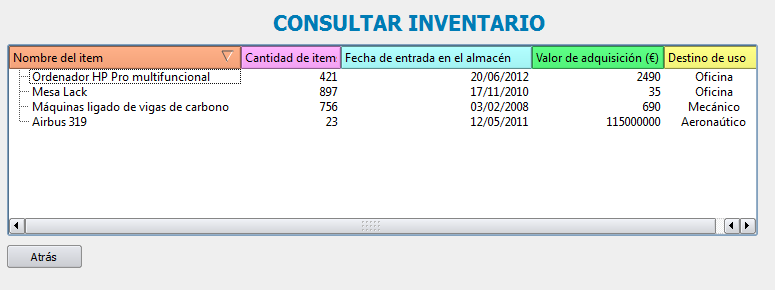
\includegraphics[scale=.6]{imagenes/consultarInventarioImagen.png}
	\caption{Pantalla aproximada de la consulta de inventario}
\end{figure}

								


				% FUNCIÓN: CONSULTAR FICHA DE EMPLEADOS
				% Caso de uso: consultar ficha empleado.
% Obs: para escribir comas en el texto del primer parámetro se han de encerrar entre {}.

% Revisado por Cristina y Juanan el día 11/03/2013

\casodeuso{
	% Nombre del caso de uso
	nombre=Consultar ficha empleado,
	% Objetivo
	objetivo={Mostrar la lista de empleados de la compañía, permitiendo buscar y filtrar resultados, así como información detallada de cada empleado en particular.},
	% Entradas
	entradas={Opcionalmente, campos de búsqueda.},
	% Precondiciones
	precondiciones=El operador de la aplicación tiene credenciales que le habilitan para realizar dicha operación.,
	% Salidas
	salidas=Lista de empleados e información detallada sobre el seleccionado.,
	% Postcondiciones en caso de éxito
	postexito=No se realiza ningún cambio en el sistema.,
	% Postcondiciones en caso de error
	posterror=No se realiza ningún cambio en el sistema.,
	% Actores
	actores={Los directivos, empleados de recursos humanos y la base de datos.}.
}{
	% Tabla de secuencia normal del caso de uso
	\begin{tablasecuencias}
		1 & Se extrae de la base de datos del sistema el listado de empleados. Si error S-1.\\
		2 & Se muestra por pantalla la lista de empleados.\\
		3 & El usuario puede filtrar los resultados y buscar empleados según diferentes criterios, como tipo de empleado, duración en la empresa, departamentos, etc.\\
		4 & Se selecciona un empleado.\\
		5 & Se muestra la información detallada del empleado. Si error S-1.
	\end{tablasecuencias}
}{
	% Tabla de secuencia con errores del caso de uso
	\begin{tablasecuencias}
		S-1 & No se puede conectar con la base de datos, se muestra un mensaje de error por pantalla dando la opción de reintentar o volver al menú principal de la aplicación.
	\end{tablasecuencias}
}

			
				% FUNCIÓN: DAR DE BAJA EMPLEADO
				
% Revisado por Cristina el día 12/03/2013

\srsfuncion{Dar de baja empleado}
	Esta función permite dar de baja a un empleado, eliminando su información personal de acuerdo a la legislación vigente y derogando las autorizaciones de acceso al sistema y las instalaciones.
	
	\begin{enumerate}
		\item \textit{Prioridad}: alta.
		\item \textit{Entradas}
		\begin{enumerate}
			\item No hay entradas.
		\end{enumerate}
		\item \textit{Flujo de operaciones}
		\begin{enumerate}
			\item El administrativo confirma que quiere realizar la operación dar de baja con el cliente\break	 seleccionado.
			\item El empleado dado de baja pierde inmediatamente todo acceso al sistema y su información personal se elimina de la base de datos de acuerdo a la legislación vigente.
			\item Se muestra un mensaje confirmando la operación.
		\end{enumerate}
		\item \textit{Respuesta a situaciones no previstas}
		\begin{enumerate}
			\item Si no se puede establecer conexión con la base de datos, se muestra un mensaje de error y se da la opción de reintentar o abortar el proceso.
		\end{enumerate}
	\end{enumerate}

			
				% FUNCIÓN: CONFIGURAR NÓMINA
				\srsfuncion{Configurar nómina}
	Función que debe permitir confeccionar y almacenar las nóminas mensuales de cada empleado de la compañía según las incidencias que se hayan producido en el último mes.
						
	\begin{enumerate}
		\item \textit{Prioridad}: alta.
		\item \textit{Entradas}
			\begin{enumerate}
				\item El usuario debe introducir en el campo de incidencias los motivos por los cuales este mes se produce una modificación en la nómina como, por ejemplo, aumentos o disminuciones del salario a causa de horas extras, comisiones, sustituciones, huelgas\ldots
				\item El sueldo del mes deberá ser mayor o igual al salario mínimo establecido por ley.
			\end{enumerate}
		\item \textit{Flujo de operaciones}
			\begin{enumerate}
				\item Una vez que el usuario ha pulsado la pestaña de \verb|Configurar nómina|, tiene que seleccionar el empleado cuya nómina ha de ser modificada. 
				\item A continuación, el usuario rellena de forma obliglatoria el campo de incidencias y confirmará que quiere aplicar los cambios en la nómina del cliente seleccionado.
				\item Por último, se registra la nómina en la base de datos.
			\end{enumerate}
		\item \textit{Respuesta a situaciones no previstas}
			\begin{enumerate}
				\item Si no se puede establecer conexión con la base de datos: se muestra un mensaje de error y se da la opción de reintentar o abortar el proceso.
				\item Si no se puede registrar la nómina: anular la operación y volver a la página principal del sistema.
			\end{enumerate}					
	\end{enumerate}
								


				% FUNCIÓN: INTRODUCIR PLAN DE VUELO
				\srsfuncion{Introducir plan de vuelo}
	Esta función debe añadir un nuevo vuelo a la lista de vuelos de la compañía aérea.

	\begin{enumerate}
		\item \textit{Entradas}
			\begin{enumerate}
				\item Los campos a introducir por el usuario son: \gls{numero_de_vuelo}, fecha y hora de origen y llegada, aeropuerto de origen y destino, el modelo de avión y el  precio total según la clase (turista, turista superior, business y primera) y tipo de pasajero (adulto, niño y bebé).
				\item El número de vuelo caracteriza e identifica unívocamente a todos los vuelos operados por la compañía. Si dicho parámetro es introducido, todos los demás deben ser ignorados en la búsqueda. Se ha de comprobar que el formato del número de vuelo se corresponde con una sucesión de 4 carácteres numéricos (si el número de caracteres es menor que 4 se completará con \verb|0| por la izquierda).
				\item No se debe permitir introducir fechas u horas no válidas.
				\item Los aeropuertos de origen y destino son un conjunto finito y han de haber sido configurados previamente. Internamente se componen de nombre, ciudad y código \gls{IATA}; externamente se visualizan como una secuencia de texto configurada. El usuario podrá seleccionar uno entre ellos para cada entrada (operación que se puede abreviar introduciendo el código IATA).
				\item El modelo de avión tiene que estar disponible en las fechas indicadas, así como en un correcto estado para su funcionamiento. Por supuesto, dicho modelo debe estar registrado en el inventario.
			\end{enumerate}
		\item \textit{Flujo de operaciones}
			\begin{enumerate}
				\item Se muestra un formulario con los campos anteriormente descritos.
				\item El usuario completa obligatoriamente todos los campos. Ningún campo permite entradas erróneas por definición, salvo el de código de aeropuertos, que tras introducir un código de aeropuerto válido lo selecciona en el \gls{combobox} de aeropuertos y si no es válido no tiene efecto alguno, restaurándose su valor original.
				\item Para cada tipo de clase y de pasajero se mostrará un botón \verb|Calcular precio| que permitirá determinar el precio del vuelo en función del pasajero.
				\item Se crea el nuevo vuelo pulsando sobre el botón \verb|Añadir vuelo|.
			\end{enumerate}
		\item \textit{Respuesta a situaciones no previstas}
			\begin{enumerate}
				\item Si no se puede acceder a la base de datos de configuraciones: no mostrar la pantalla de inicio de la función e informar del error al usuario.
				\item Si alguno de los datos es erróneo: informar al usuario y volver a solicitar la información.
			\end{enumerate}
	\end{enumerate}
	\begin{figure}[ht]\centering
	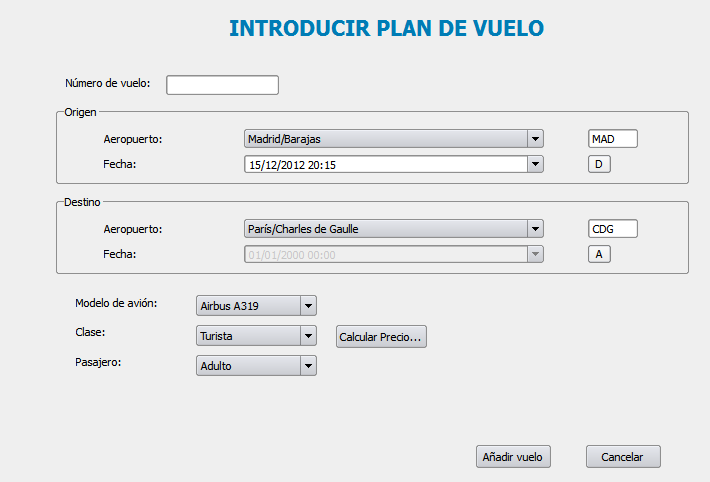
\includegraphics[scale=.6]{imagenes/introducirPlanDeVueloImagen.png}
	\caption{Pantalla aproximada de como introducir un nuevo vuelo}
\end{figure}

				
				% FUNCIÓN: FACTURAR
				\srsfuncion{Facturar}
	Esta función debe controlar la facturación del equipaje del viajero.

	\begin{enumerate}
		\item \textit{Prioridad}: alta.
		\item \textit{Entradas}
			\begin{enumerate}
				\item Los campos a introducir por el usuario son: \gls{numero_de_vuelo}, número de reserva y peso del equipaje.
				\item El número de vuelo caracteriza e identifica unívocamente a todos los vuelos operados por la compañía.
				\item El peso del equipaje debe ser expresado en kilogramos. En caso de que dicha cantidad supere el máximo permitido por billete, el pasajero deberá pagar la cantidad de dinero que indique el sistema. En cualquier caso, el peso del equipaje deberá estar dentro de un rango establecido previamente por la compañía.
			\end{enumerate}
		\item \textit{Flujo de operaciones}
			\begin{enumerate}
				\item Se muestra un formulario con el número de vuelo, número de reserva y peso del equipaje.
				\item El usuario completa obligatoriamente todos los campos. Si el peso excede el permitido por billete, se indicará la cantidad a pagar y se habilitará un botón \verb|Confirmar pago| para indicar al sistema que el cliente ha abonado el dinero por el exceso de equipaje. No se dejará continuar mientras no se pulse dicha opción o no se modifique el peso del equipaje.
				\item Cuando los datos sean correctos, el usuario deberá pulsar el boton de \verb|Facturar| para confirmar la operación.
			\end{enumerate}
		\item \textit{Respuesta a situaciones no previstas}
			\begin{enumerate}
				\item Si alguno de los datos introducidos no es válido: se muestran los campos erróneos y se da la opción de modificarlos.
				\item Si no se puede acceder a la base de datos: se muestra un mensaje de error y vuelve a la página anterior.
			\end{enumerate}
	\end{enumerate}	

			
				% FUNCIÓN: EFECTUAR EMBARQUE
				% Caso de uso: Efectuar embarque
% Obs: para escribir comas en el texto del primer parámetro se han de encerrar entre {}.

% Comentario de Aitor, si un cliente no se presenta a un embarque se cancelan todos los billetes asociados a ese cliente.
% Revisado por Juanan el día 12/03/2013

\casodeuso{
	% Nombre del caso de uso
	nombre=Efectuar embarque,
	% Objetivo
	objetivo=Registrar el embarque del pasajero.,
	% Entradas
	entradas=El número de vuelo y el número de reserva del pasajero.,
	% Precondiciones
	precondiciones=El operador de la aplicación tiene credenciales que le habilitan para realizar dicha operación y un billete válido,
	% Salidas
	salidas=Confirmación de que el pasajero pasa el control de seguridad con éxito y ha embarca en el avión.,
	% Postcondiciones en caso de éxito
	postexito=Se registra el embarque del pasajero.,
	% Postcondiciones en caso de error
	posterror=No se realiza ningún cambio en el sistema.,
	% Actores
	actores=El personal de la compañía presente en el aeropuerto y la base de datos.
}{
	% Tabla de secuencia normal del caso de uso
	\begin{tablasecuencias}
		1 & El usuario introduce el número de vuelo y el número de reservar del pasajero. Si error S-1.\\
		2 & Se comprueba la reserva y se actualiza la base de datos. Si error S-2.		
	\end{tablasecuencias}
}{
	% Tabla de secuencia con errores del caso de uso
	\begin{tablasecuencias}
		S-1 & Alguno de los campos introducidos por el usuario no es válido. Se muestra un mensaje de error y se vuelve a 1 de la secuencia normal de uso indicando los datos erroneos. \\
		S-2 & No se ha podido conectar con la base de datos. Se muestra un mensaje de error y se ofrece la posibilidad de reintentar.
	\end{tablasecuencias}
}



				% FUNCIÓN: EFECTUAR EMBARQUE
				% Caso de uso: ver incidencias del sistema.
% Obs: para escribir comas en el texto del primer parámetro se han de encerrar entre {}.

\casodeuso{
	% Nombre del caso de uso
	nombre=Ver incidencias del sistema,
	% Objetivo
	objetivo={Permite a los supervisores informáticos del sistema inspeccionar el correcto funcionamiento del \software y responder a comportamientos erróneos del mismo que hayan sido detectados, a partir de los registros que este genera.},
	% Entradas
	entradas={El nombre de registro que se quiere consultar.},
	% Precondiciones
	precondiciones={El operador de la aplicación está debidamente registrado y posee credenciales que le habilitan para realizar esta operación.},
	% Salidas
	salidas={Archivos de registro del sistema solicitados.},
	% Postcondiciones en caso de éxito
	postexito={},
	% Postcondiciones en caso de error
	posterror={El sistema central no habrá sufrido cambios.},
	% Actores
	actores={Personal de \textit{Servicios Informáticos} y supervisores del sistema con autorización para ello.},
}{
	% Tabla de secuencia normal del caso de uso
	\begin{tablasecuencias}
		1 & Los archivos de registro del servidor central y los errores reportados por las aplicaciones cliente componen una serie de archivos de texto en el servidor central. Esos archivos podrán ser consultados dando acceso a su ubicación en el sistema de archivos del servidor central.
		% De momento, ¿para qué complicarlo?
	\end{tablasecuencias}
}{
	% Tabla de secuencia con errores del caso de uso
	\begin{tablasecuencias}
		S-1 & Las secuencias alternativas son las que determine el método de acceso al servidor.
	\end{tablasecuencias}
}


			\subsubsection{Gestión externa}
				% FUNCIÓN: ACCEDER GESTIÓN EXTERNA
				% Revisado por Cristina el día 12/03/2013

\srsfuncion{Acceder web} \label{fun:accederge}
	Función que permite hacer \textit{\gls{Login}} al usuario (en este caso cliente de la compañía aérea) para poder acceder al sistema.
		
	\begin{enumerate}
		\item \textit{Prioridad}: media.
		\item \textit{Entradas}
		\begin{enumerate}
			\item El nombre de usuario y la contraseña son campos obligatorios a introducir.
			\item En el campo contraseña son válidos los caracteres ASCII imprimibles.
		\end{enumerate}
		\item \textit{Flujo de operaciones}
		\begin{enumerate}
			\item Se muestran por pantalla dos campos a rellenar: uno para introducir el id del usuario y otro para escribir la contraseña.
			\item El usuario selecciona la opción de acceder al sistema.
		\end{enumerate}
		\item \textit{Respuesta a situaciones no previstas}
		\begin{enumerate}
			\item Si algún campo introducido no es válido, se indica y se da la opción de introducirlo de nuevo. Existe un límite de 5 intentos de acceso fallido en un periodo de tiempo corto (15 minutos).
		\end{enumerate}
	
\end{enumerate}


				% FUNCIÓN: REGISTRARSE
				
% Revisado por Juanan el día 12/03/2013

\srsfuncion{Registrarse} \label{fun:registrarse}
	Esta función crea una nueva cuenta de cliente asociada a un visitante de la página web de la compañía.

	\begin{enumerate}
		\item \textit{Prioridad}: alta.
		\item \textit{Entradas}\\
			Será necesario introducir los siguiente datos: nombre y apellidos, código de identificación personal y una cuenta de correo electrónico. En cambio, la introducción de los siguientes datos es opcional: teléfono, dirección.

			\begin{enumerate}
				\item El código de idenficación personal será validado de acuerdo a las especificaciones de su formato.
				\item El nombre y los apellidos deberán contener únicamente carácteres alfabéticos latinos, acentuados o no, y espacios.
				\item La dirección de correo ha de seguir el formato \verb|nombre@dominio.com|. Se comprobará, en la medida de los posible, la autenticidad del servicio de correo introducido.
				\item El número de teléfono debe ser una secuencia de 9 dígitos. % Telefono español?
				\item La dirección debe cumplir los requisitos establecidos en \nameref{srs:direccionpostal}.
			\end{enumerate}
		
		\item \textit{Flujo de operaciones}
			\begin{enumerate}
				\item Se muestra un formulario con los distintos campos anteriormente detallados para que el usuario los rellene. 
				\item Se solicita además el paso de un \gls{captcha} por motivos de seguridad. Hasta que éste no sea superado no se permitirá continuar con el registro.
				\item Se muestran los derechos del usuario y las condiciones del servicio que deberán ser aceptadas, no pudiendo seguir con el registro hasta entonces.
				\item Cuando ha realizado correctamente todos los pasos anteriores debe \verb|Confirmar registro| y se procede al registro en la base de datos central.
			\end{enumerate}
		\item \textit{Respuesta a situaciones no previstas}
			\begin{enumerate}
				\item Si alguno de los datos no es válido o se ha dejado sin rellenar algún campo obligatorio se mostrará como erróneo y se dará la opción al usuario de modificarlo.
				\item Si no se puede registrar al usuario en la base de datos: informar al usuario e indicarle que puede volverlo a intentar en otro momento.
			\end{enumerate}
		\item \textit{Relación con otras funciones}\\
			Este caso es útil para todos aquellos que requieran un usuario registrado, como \verb|Acceder web| o aunque no lo requieran como \nameref{fun:iniciarpago}.
	\end{enumerate}


				% FUNCIÓN: EDITAR CLIENTE
				\srsfuncion{Editar cliente} \label{fun:editarcliente}
	Esta función debe mostrar al usuario su perfil y permitirle la modificación del mismo.

\begin{enumerate}
	\item \textit{Entradas}
	\begin{enumerate}
		\item Las opciones que admiten modificación son: Contraseña, domicilio, dirección de correo electrónico, tarjeta de crédito asociada.
		\item La contraseña estará formada por entre 8 y 16 caracteres alfanúmericos.
		\item El código postal del domicilio ha de estar formado por 5 cifras.
		\item Se comprobará la correción del correo electrónico mediante un e-mail de verificación.
		\item Se verificará algoritmicamente los 20 digitos de numeración de la tarjeta de crédito, así como la validez de la misma junto con la fecha de caducidad y el código \gls{CVV2}.
	\end{enumerate}
	\item \textit{Flujo de operaciones}
	\begin{enumerate}
		\item Se muestra un formulario con los campos modificables actuales del usuario.
		\item El usuario modifica al menos uno de los diferentes campos. La válided de los campos modificados se comprueba al pulsar el botón Guardar Cambios.
		\item Si se encuentra algún dato erroneo se informa de ello. Si se verificán los datos modificados se confirma la operación, actualizando la \gls{base_de_datos}.
		\item Se muestra el perfil de usuario resultado de la modificación.
	\end{enumerate}
	\item \textit{Respuesta a situaciones no previstas}
	\begin{enumerate}
		\item Si no se puede acceder o modificar a la base de datos: informa de la no disponibilidad temporal al usuario.
	\end{enumerate}
\end{enumerate}


				% FUNCIÓN: VER INFORMACIÓN DE VUELO
				% Caso de uso: ver información de vuelo
% Obs: para escribir comas en el texto del primer parámetro se han de encerrar entre {}.

\casodeuso{
	% Nombre del caso de uso
	nombre=Ver información de vuelo contratado,
	% Objetivo
	objetivo=Mostrar al usuario la información de sus vuelos contratados.,
	% Entradas
	entradas=,
	% Precondiciones
	precondiciones=El usuario ha iniciado sesión correctamente en la interfaz web.,
	% Salidas
	salidas=Información detallada de la reserva(número de vuelo, fecha y hora, número de plaza, terminales de salida y de llegada\ldots)},
	% Postcondiciones en caso de éxito
	postexito=No se realiza ningún cambio en el sistema.,
	% Postcondiciones en caso de error
	posterror=No se realiza ningún cambio en el sistema.,
	% Actores
	actores=Cliente-usuario de interfaz web.
}{
	% Tabla de secuencia normal del caso de uso
	\begin{tablasecuencias}
		1 & Muestra listado detallo de los vuelos contratados. Si no disponibles S-1.\\
		2 & Ofrece la opción de seleccionar e imprimir la información de los vuelos mostrados.
	\end{tablasecuencias}
}{
	% Tabla de secuencia con errores del caso de uso
	\begin{tablasecuencias}
		S-1 & Si no se puede conectar con la base de datos se muestra mensaje  de tipo \textit{información no disponible temporalmente} y se vuelve al menú principal de la aplicación.
	\end{tablasecuencias}
}


				% FUNCIÓN: MOSTRAR OFERTAS
				\srsfuncion{Mostrar ofertas} \label{fun:mostrarofertas}
	Esta función debe mostrar las ofertas que tiene la compañía en estos momentos.
	
\begin{enumerate}
	\item \textit{Prioridad}: media.
	\item \textit{Entradas}
	\begin{enumerate}
		\item Se mostrarán las ofertas adaptadas al idioma que tenga la página web y el cliente.
		\item Esas ofertas tendrán que ser accesibles para el usuario en el momento en que se le muestran.
	\end{enumerate}
	\item \textit{Flujo de operaciones}
	\begin{enumerate}
		\item Se mostrará el resumen de cada oferta. Este consta de la información importante que la empresa ha decidido destacar en la oferta. 
		\item El cliente podrá elegir si desea ver detalladamente la información de la oferta.
	\end{enumerate}
	\item \textit{Respuesta a situaciones no previstas}
	\begin{enumerate}
		\item En caso de no poder acceder a la base de datos para obtener las ofertas, se actuará como si no hubiese ofertas disponibles en este momento y se continuará el proceso de forma normal.
	\end{enumerate}
\end{enumerate}

				
				% FUNCIÓN: CONSULTAR OFERTA
				% Caso de uso: Consultar oferta.
% Obs: para escribir comas en el texto del primer parámetro se han de encerrar entre {}.

% Revisado por Cristina el día 11/03/2013
% Nombre antiguo: accederaUnaOferta

\casodeuso{
	% Nombre del caso de uso
	nombre=Consultar oferta,
	% Objetivo
	objetivo=Consultar una oferta elegida por el cliente.,
	% Entradas
	entradas=No hay entradas.,
	% Precondiciones
	precondiciones=No hay precondiciones.,
	% Salidas
	salidas=Los detalles de una oferta específica.,
	% Postcondiciones en caso de éxito
	postexito=No se realiza ningún cambio en el sistema.,
	% Postcondiciones en caso de error
	posterror=No se realiza ningún cambio en el sistema.,
	% Actores
	actores=Los clientes de la compañía y la base de datos.,
}{
	% Tabla de secuencia normal del caso de uso
	\begin{tablasecuencias}
		1 & Se extrae de la base de datos la información completa de la oferta. Si error S-1.
	\end{tablasecuencias}
}{
	% Tabla de secuencia con errores del caso de uso
	\begin{tablasecuencias}
		S-1 & No se puede conectar con la base de datos, se muestra un mensaje de error por pantalla dando la opción de reintentar o volver al menú principal de la aplicación.
	\end{tablasecuencias}
}


				% FUNCIÓN: INICIAR PAGO BILLETES
				\srsfuncion{Iniciar pago billetes de vuelo} \label{fun:iniciarpago}
	Esta función debe permitir al usuario adquirir un billete de vuelo, de acuerdo a la selección previa.

\begin{enumerate}
	\item \textit{Entradas}
	\begin{enumerate}
		\item Los detalles completos de la selección del vuelo.
	\end{enumerate}
	\item \textit{Flujo de operaciones}
	\begin{enumerate}
		\item Se muestra por pantalla los datos completos del vuelo, siempre que no se haya excedido el tiempo de reserva desde la selección del billete.
		\item Se muestra las claúsulas de las leyes de protección de datos para que el usuario las acepte. Hasta que no lo haga no continúa el proceso de pago.
		\item Se redirecciona a \nameref{fun:pagotarjeta}.
	\end{enumerate}
	\item \textit{Respuesta a situaciones no previstas}
	\begin{enumerate}
		\item Si no se puede acceder a la base de datos para almacenar la información: se muestra un mensaje de error por pantalla informando de que el proceso de pago se ha interrumpido. Se vuelve a la página anterior.
	\end{enumerate}
\end{enumerate}


				% FUNCIÓN: PAGO TARJETA
				% Revisado por Juanan el día 12/03/2013

\srsfuncion{Realizar pago con tarjeta} \label{fun:pagotarjeta}
	Esta función permite al usuario finalizar el proceso de compra del billete realizando el pago con tarjeta de crédito o débito.

\begin{enumerate}
	\item \textit{Prioridad}: alta.
	\item \textit{Entradas}
	\begin{enumerate}
		\item El nombre del usuario (nombre y apellidos) deberán contener únicamente carácteres\break alfabéticos latinos, acentuados o no, y espacios.
		\item El número de la tarjeta deberá ser una secuencia de 4 bloques de 4 dígitos, todos ellos enteros mayores o iguales que 0.
		\item El código CCV deberá ser una secuencia de 3 dígitos mayores o iguales que 0.
		\item La fecha de caducidad  ser una secuencia de 5 caracteres compuesta por: 2 dígitos para indicar el mes (en el rango 01-12) , una barra `/'  y otros 2 dígitos para indicar el año, que serán las dos últimas cifras del mismo.
	\end{enumerate}
	\item \textit{Flujo de operaciones}
	\begin{enumerate}
		\item Se muestra por pantalla una tabla con los datos de la tarjeta a completar (nombre y apellidos, número, código CCV y fecha de caducidad). Una vez completos, se habilita la opción \verb|Confirmar|.
		\item Se transfieren los datos de la tarjeta a la empresa emisora de las mismas para que compruebe si los datos son correctos y la tarjeta está operativa. En este caso, se enviará al instante un mensaje a la compañía indicando que los datos introducidos por el usuario son válidos.
		\item Si está todo correcto, se da la opción de imprimir en el momento la tarjeta de embarque o guardarla como pdf para imprimirla en otro momento.
	\end{enumerate}
	\item \textit{Respuesta a situaciones no previstas}
	\begin{enumerate}
		\item Si no se puede acceder a la base de datos para almacenar la información: se muestra un mensaje de error por pantalla informando de que el proceso de pago se ha interrumpido. Se vuelve a la página anterior.
		\item Si alguno de los datos no es válido: se muestran los campos erróneos y se da la opción de editarlos de nuevo.
		\item Si algún campo no se ha rellenado: se muestra un mensaje indicando que es obligatorio completarlo.
		\item Si la tarjeta está inhabilitada por algún motivo: se muestra un error indicando que el pago no ha podido completarse porque la tarjeta está bloqueada. Se cancela la operación y se vuelve a la página principal de la aplicación.
		\item Si los datos de la tarjeta no son válidos: se muestra un error indicando que el pago no ha podido completarse y se da la opción al usuario de modificar los datos introducidos al principio de la operación.
	\end{enumerate}
	\item \textit{Relación con otras funciones}\\
		Esta función está relacionada con \nameref{fun:consultaroferta}, \nameref{fun:mostrarofertas}, \nameref{fun:iniciarpago} y \nameref{fun:comprarbillete}.	
\end{enumerate}


				% FUNCIÓN: PRESENTAR RECLAMACIÓN
				% Caso de uso: Presentar reclamacion
% Obs: para escribir comas en el texto del primer parámetro se han de encerrar entre {}.

\casodeuso{
	% Nombre del caso de uso
	nombre=Presentar reclamaciones,
	% Objetivo
	objetivo= Presentar una reclamación por parte del cliente.,
	% Entradas
	entradas= Motivo de la queja y detallado de la misma.,
	% Precondiciones
	precondiciones=Intención por parte del usuario de transmitir una sugerencia o queja a la empresa.,
	% Salidas
	salidas=Confirmación del envio y número asociado a la reclamación.,
	% Postcondiciones en caso de éxito
	postexito=La notificación es enviada correctamente al departamento correspondiente.,
	% Postcondiciones en caso de error
	posterror=No se tramita la petición.,
	% Actores
	actores=Cliente-usuario de interfaz web.,
}{
	% Tabla de secuencia normal del caso de uso
	\begin{tablasecuencias}
		1 & Completar todos sus datos, el motivo de la reclamación, y detalles de la misma. Si error S-1. \\
		2 & Muestra número asignado a la reclamación junto a la confirmación de que la reclamación ha sido tramitada y en breve será atendia por el departamento correspondiente. Si error S-2. 
		
	\end{tablasecuencias}
}{
	% Tabla de secuencia con errores del caso de uso
	\begin{tablasecuencias}
		S-1 & Los campos de datos están incompletos. Indicar los campos erróneos o vacíos.\\
		S-2 & Si no se han podido transmitir los datos de la reclamación a nuestra base de datos se indicará un mensaje de que la operación ha sido fallida debido a errores técnicos y de que se vuelva a intentar.
	\end{tablasecuencias}
}


						
				% FUNCIÓN: COMPRAR BILLETE
				\srsfuncion{Comprar billete}
	Esta función debe permitir al usuario iniciar el proceso de compra de billetes de un vuelo seleccionado.		

	\begin{enumerate}
		\item \textit{Entradas}
			\begin{enumerate}
				\item El nombre y apellidos de los pasajeros deberá contener únicamente carácteres alfabéticos latinos, acentuados o no, y espacios.
				\item La selección de asientos se realizará en función de los asientos disponibles en el momento de la compra de los billetes.
				\item Los datos de la persona que paga serán, de momento, nombre y apellidos,  que deberá contener únicamente carácteres alfabéticos latinos, acentuados o no, y espacios.							
			\end{enumerate}
		\item \textit{Flujo de operaciones}
			\begin{enumerate}
				\item Se muestra por pantalla el itinerario del vuelo a comprar, el precio total a pagar, desglosándolo en la parte correspondiente al pasajero, la tarifa, los impuestos, tasas y suplementos de transporte.
				\item Se muestran los asientos disponibles del avión en el momento de la compra, dando la opción al cliente de reservar los asientos que desee en su vuelo.
				\item El cliente deberá introducir los datos (nombre y apellidos) de la persona que realizará el pago de billetes (no tiene porqué ser un pasajero). Si todo ha ido correctamente se habilita un botón \verb|Continuar| y se redirecciona a~\ref{fun:iniciarpago}.
			\end{enumerate}
		\item \textit{Respuesta a situaciones no previstas}
			\begin{enumerate}
				\item Si no se puede mostrar la información del vuelo seleccionado: se muestra un mensaje de error por pantalla y se vuelve a la página anterior.
				\item Si alguno de los datos no es válido: se muestran los campos erróneos y se da la opción de editarlos de nuevo.
				\item Si algún campo no se ha rellenado: se muestra un mensaje indicando que es obligatorio completarlo.
				\item Si no se puede realizar la reserva de asientos: se muestra el error y sigue la secuencia normal.
				\item Si no se puede conectar con la base de datos y, por tanto, no se puede realizar la compra,  se mostrará un mensaje indicando que el proceso de pago ha sido interrumpido. Se vuelve a la página principal de la aplicación.
			\end{enumerate}
	\end{enumerate}
								


				% FUNCIÓN: CONSULTAR VUELO
				% Caso de uso: consultar vuelo.
% Obs: para escribir comas en el texto del primer parámetro se han de encerrar entre {}.

% Revisado por Cristina el día 11/03/2013

\casodeuso{
	% Nombre del caso de uso
	nombre=Consultar vuelo,
	% Objetivo
	objetivo={Mostrar al cliente la relación de vuelos operados por la compañía, permitiendo buscar y filtrar resultados, así como información detallada de un vuelo en particular.},
	% Entradas
	entradas={Opcionalmente, campos de búsqueda(aeropuertos de origen y destino, número de escalas, fecha y hora, precio del billete\ldots).},
	% Precondiciones
	precondiciones=No hay precondiciones.,
	% Salidas
	salidas=Lista de vuelos e información detallada sobre el seleccionado.,
	% Postcondiciones en caso de éxito
	postexito=No se realiza ningún cambio en el sistema.,
	% Postcondiciones en caso de error
	posterror=No se realiza ningún cambio en el sistema.,
	% Actores
	actores=Los clientes de la compañía y la base de datos.,
}{
	% Tabla de secuencia normal del caso de uso
	\begin{tablasecuencias}
		1 & Se extrae de la base de datos del sistema el listado de vuelos. Si error S-1.\\
		2 & Se muestra la lista de vuelos ordenada por un criterio asignado por defecto.\\
		3 & El usuario puede filtrar los resultados y buscar vuelos según diferentes criterios.\\
		4 & Se selecciona un vuelo.\\
		5 & Se muestra la información detallada del vuelo. Si error S-1.
	\end{tablasecuencias}
}{
	% Tabla de secuencia con errores del caso de uso
	\begin{tablasecuencias}
		S-1 &No se puede conectar con la base de datos, se muestra un mensaje de error por pantalla dando la opción de reintentar o volver al menú principal de la aplicación.
	\end{tablasecuencias}
}


		% Termina el índice parcial para funciones
		\stopcontents[tocfunciones]

		\subsection{Requisitos de rendimiento}
			% Los números son completamente inventados.
			El sistema interno deberá reconocer y soportar hasta 4.000 terminales, si bien en determinadas circunstancias agrupaciones de terminales podrían comportarse como uno sólo, gestionándose \textit{in situ} esa eventualidad. El sistema deberá soportar hasta 1.000 usuarios conectados simultáneamente a aquellos servicios del \software de gestión interna que requieran una conexión latente (\textit{KeepAlive}) con el servidor central, ampliándose ese límite a 2.000 al considerar las conexiones de corta duración. Además, el 90\% de las transacciones deberán realizarse en menos de un minuto. La interfaz de gestión interna o servidor web admitirá hasta 6.000 conexiones simultáneas para el contenido estático, si bien el número de conexiones para contenido dinámico estará sometido a los límites marcados por el sistema de gestión interna.\\

			% Los requisitos provienen de los requisitos de Windows Xp.
			Los requisitos de rendimiento de los equipos sobre los que se ejecute la aplicación de \textit{Gestión Interna} demandan los siguientes requisitos de \hardware{}:
				\begin{itemize}
					\item Procesador \textit{Pentium} o equivalente a un mínimo de 233 MHz.
					\item 128 Mb de memoria RAM con velocidad de transferencia de más de 250 MHz.
					\item 10 GB disponibles en el disco duro a una tasa de transferencia superior a 10 MBit/s.
					\item Adaptador de vídeo igual o superior a \textit{Nvidia GeForce 256} o equivalente.
				\end{itemize}

			Bastará con una intensidad media de conexión a Internet para la \textit{Gestión Externa} de la compañía.\\

			La base de datos es un elemento crítico en el rendimiento del sistema. Se prevén realizar miles de interacciones al día, por lo que debe ofrecer alta disponibilidad.

		\subsection{Requisitos lógicos de la base de datos}
			Los requisitos lógicos para las funciones que trabajan con la base de datos son:
			\begin{itemize}
				\item \textbf{Tipos de información usada por diversas funciones: } Existen funciones que recibirán cadenas de texto, unas que las usarán para mostrar los datos por pantalla para que el usuario de la aplicación pueda observar la información, y otras que las recibirán para cubrir las necesidades ya que la acción que realiza requiere de dichos datos. En el primer tipo de funciones, existen varias que podrán recibir además imágenes como complemento para mostrar la información.
				\item \textbf{Frecuencia de uso: } Las funciones tienen distintas frecuencias de acceso a la base de datos, existiendo algunas en las que se acceda en escasas ocasiones y en momentos específicos como pueden ser \nameref{fun:configSystem}, Organizar puestos de trabajo, Modificar empleados, etc., mientras que otras funciones como Acceder en gestión interna o Consultar Vuelo tendrán una alta frecuencia de acceso a la base de datos.
				\item \textbf{Capacidades de acceso: } Las funciones del sistema deben tener unas capacidades de acceso muy diferentes ya que costes como el que ocasiona la búsqueda un cliente específico entre todos los que están en la base de datos son mucho mayores que otros, como puede ser el de mostrar la información económica de la empresa. Por ello, una información tendrá que ser más accesible y fácil de encontrar para unas funciones, y así facilitarle el trabajo, por ejemplo, al que tenga que realizar la tarea de buscar un cliente o empleado específico. 
				\item \textbf{Entidades de datos y sus relaciones: } Los datos almacenados deben cumplir unas condiciones prefijadas para posibilitar su correcto uso por el sistema y que dependerán de la entidad de datos a la que correspondan. Además, algunos datos estarán estrechamente relacionados con otros como puede ser las ofertas y los vuelos disponibles, o incluso los incluirán como los datos de los empleados de la empresa incluyen la información relativa a sus horarios y nóminas.
			\end{itemize}

		\subsection{Restricciones de diseño}
			El diseño de este producto está condicionado por la naturaleza y los usos del cliente, de lo que se derivan algunas limitaciones. La existencia previa de un parque de equipos informáticos distribuidos en las instalaciones de la compañía que el cliente quiere conservar imponen la necesidad de acomodar el \software a las posibilidades que ofrecen dichas máquinas. Este en particular, no plantea grandes problemas, ya que la aplicación cliente para la gestión interna --que será instalada en esos equipos-- no exige atributos que no estén presentes en la mayoría de las máquinas; si bien la obsolescencia de algunos equipos puede dejar sin efecto los requisitos de rendimiento indicados en el texto. Por otro lado, el amplio uso de ordenadores compartidos en ciertos sectores de la compañía ha impuesto limitar el almacenamiento local de información. Así mismo, la expansión internacional del cliente y las diferentes legislaciones sobre tratamiento de datos de carácter personal restringen posibles características del producto.
			\subsubsection{Cumplimiento de estándares}
				Este producto ha sido diseñado de acuerdo a ciertos estándares sobre materias diversas.\\
				
				En el terreno económico y financiero, toda operación realizada por la aplicación es conforme a las \gls{NIC} \cite{NIC2006} y especialmente al \textit{Plan General de Contabilidad} de España \cite{PGC2007}.\\

				En el ámbito de la actividad del cliente, se han seguido recomendaciones y estándares relevantes de la \gls{IATA}.
				
		\subsection{Atributos del sistema software}
			El diseño del sistema se ha basado en características como:
			\begin{itemize}
				\item \textit{Seguridad}: implementando sistemas para evitar fraude, sistemas seguros y de encriptado para cobro, procesos de identificación de empleados basados en niveles de acceso y secciones.
				\item \textit{Estabilidad}: es fundamental la protección del sistema frente a errores, manteniendo en todo momento copias de seguridad de las bases de datos y registrando accesos y modificaciones.
				\item \textit{\gls{Usabilidad}}: pone al alcance del usuario una interfaz gráfica relativamente sencilla e intuitiva pero a la vez completa.
				\item \textit{Escalabilidad}: se desarrolla el sistema facilitando el mantenimiento del mismo así como la posibilidad de ampliaciones y nuevas funcionalidades futuras.
			\end{itemize}
	
	% Apéndice: Glosario
	\newpage
	\appendix
	\section{Apéndice: Glosario} \label{srs:glosario}
	\printglossary 

	% Subíndice de funciones
	\newpage
	\printcontents[tocfunciones]{}{2}{\section{Lista de funciones}\setcounter{tocdepth}{4}}

	\newpage
	\listoffigures

	\newpage
	\nocite{IEEE:1074}
	\nocite{IEEE:830}
	\bibliography{srs}
	\bibliographystyle{plain}
	
	\listoftodos
\end{document}
